\documentclass[10pt]{beamer}
\usepackage{ragged2e} % \justifying
\usepackage[export]{adjustbox} % left and right in images
\usepackage{subcaption} % subfigure
\usepackage[none]{hyphenat} % Avoids to go out of margin

% Math symbols:
%%%%%%% Mathematical Symbols ==>>

\def\tr{^T}
\def\trd{{}^T}
\def\Atan{\mathrm{Atan2}}
\def\Acos{\mathrm{Acos}}
\def\sgn{\mathrm{sgn}}
\def\de{\mathrm{d}}
\def\diag{\mathrm{diag}}

\def\zero{\hbox{\bf 0}}
\def\Zero{{\mbox{\boldmath $O$}}}

\def\bfa{{\mbox{\boldmath $a$}}}
\def\bfb{{\mbox{\boldmath $b$}}}
\def\bfc{{\mbox{\boldmath $c$}}}
\def\bfd{{\mbox{\boldmath $d$}}}
\def\bfe{{\mbox{\boldmath $e$}}}
\def\bff{{\mbox{\boldmath $f$}}}
\def\bfg{{\mbox{\boldmath $g$}}}
\def\bfh{{\mbox{\boldmath $h$}}}
\def\bfi{{\mbox{\boldmath $i$}}}
\def\bfj{{\mbox{\boldmath $j$}}}
\def\bfk{{\mbox{\boldmath $k$}}}
\def\bfl{{\mbox{\boldmath $l$}}}
\def\bfm{{\mbox{\boldmath $m$}}}
\def\bfn{{\mbox{\boldmath $n$}}}
\def\bfo{{\mbox{\boldmath $o$}}}
\def\bfp{{\mbox{\boldmath $p$}}}
\def\bfq{{\mbox{\boldmath $q$}}}
\def\bfr{{\mbox{\boldmath $r$}}}
\def\bfs{{\mbox{\boldmath $s$}}}
\def\bft{{\mbox{\boldmath $t$}}}
\def\bfu{{\mbox{\boldmath $u$}}}
\def\bfv{{\mbox{\boldmath $v$}}}
\def\bfw{{\mbox{\boldmath $w$}}}
\def\bfx{{\mbox{\boldmath $x$}}}
\def\bfy{{\mbox{\boldmath $y$}}}
\def\bfz{{\mbox{\boldmath $z$}}}
\def\bfA{{\mbox{\boldmath $A$}}}
\def\bfB{{\mbox{\boldmath $B$}}}
\def\bfC{{\mbox{\boldmath $C$}}}
\def\bfD{{\mbox{\boldmath $D$}}}
\def\bfE{{\mbox{\boldmath $E$}}}
\def\bfF{{\mbox{\boldmath $F$}}}
\def\bfG{{\mbox{\boldmath $G$}}}
\def\bfH{{\mbox{\boldmath $H$}}}
\def\bfI{{\mbox{\boldmath $I$}}}
\def\bfJ{{\mbox{\boldmath $J$}}}
\def\bfK{{\mbox{\boldmath $K$}}}
\def\bfL{{\mbox{\boldmath $L$}}}
\def\bfM{{\mbox{\boldmath $M$}}}
\def\bfN{{\mbox{\boldmath $N$}}}
\def\bfO{{\mbox{\boldmath $O$}}}
\def\bfP{{\mbox{\boldmath $P$}}}
\def\bfQ{{\mbox{\boldmath $Q$}}}
\def\bfR{{\mbox{\boldmath $R$}}}
\def\bfS{{\mbox{\boldmath $S$}}}
\def\bfT{{\mbox{\boldmath $T$}}}
\def\bfU{{\mbox{\boldmath $U$}}}
\def\bfV{{\mbox{\boldmath $V$}}}
\def\bfW{{\mbox{\boldmath $W$}}}
\def\bfX{{\mbox{\boldmath $X$}}}
\def\bfY{{\mbox{\boldmath $Y$}}}
\def\bfZ{{\mbox{\boldmath $Z$}}}

\def\bfGamma{{\mbox{\boldmath $\Gamma$}}}
\def\bfDelta{{\mbox{\boldmath $\Delta$}}}
\def\bfTheta{{\mbox{\boldmath $\Theta$}}}
\def\bfLambda{{\mbox{\boldmath $\Lambda$}}}
\def\bfXi{{\mbox{\boldmath $\Xi$}}}
\def\bfPi{{\mbox{\boldmath $\Pi$}}}
\def\bfSigma{{\mbox{\boldmath $\Sigma$}}}
\def\bfUpsilon{{\mbox{\boldmath $\Upsilon$}}}
\def\bfPhi{{\mbox{\boldmath $\Phi$}}}
\def\bfPsi{{\mbox{\boldmath $\Psi$}}}
\def\bfOmega{{\mbox{\boldmath $\Omega$}}}
\def\bfalpha{{\mbox{\boldmath $\alpha$}}}
\def\bfbeta{{\mbox{\boldmath $\beta$}}}
\def\bfgamma{{\mbox{\boldmath $\gamma$}}}
\def\bfdelta{{\mbox{\boldmath $\delta$}}}
\def\bfepsilon{{\mbox{\boldmath $\epsilon$}}}
\def\bfzeta{{\mbox{\boldmath $\zeta$}}}
\def\bfeta{{\mbox{\boldmath $\eta$}}}
\def\bftheta{{\mbox{\boldmath $\theta$}}}
\def\bfiota{{\mbox{\boldmath $\iota$}}}
\def\bfkappa{{\mbox{\boldmath $\kappa$}}}
\def\bflambda{{\mbox{\boldmath $\lambda$}}}
\def\bfmu{{\mbox{\boldmath $\mu$}}}
\def\bfnu{{\mbox{\boldmath $\nu$}}}
\def\bfxi{{\mbox{\boldmath $\xi$}}}
\def\bfpi{{\mbox{\boldmath $\pi$}}}
\def\bfrho{{\mbox{\boldmath $\rho$}}}
\def\bfsigma{{\mbox{\boldmath $\sigma$}}}
\def\bftau{{\mbox{\boldmath $\tau$}}}
\def\bfupsilon{{\mbox{\boldmath $\upsilon$}}}
\def\bfphi{{\mbox{\boldmath $\phi$}}}
\def\bfchi{{\mbox{\boldmath $\chi$}}}
\def\bfpsi{{\mbox{\boldmath $\psi$}}}
\def\bfomega{{\mbox{\boldmath $\omega$}}}
\def\bfvarepsilon{{\mbox{\boldmath $\varepsilon$}}}
\def\bfvartheta{{\mbox{\boldmath $\vartheta$}}}
\def\bfvarpi{{\mbox{\boldmath $\varpi$}}}
\def\bfvarrho{{\mbox{\boldmath $\varrho$}}}
\def\bfvarsigma{{\mbox{\boldmath $\varsigma$}}}
\def\bfvarphi{{\mbox{\boldmath $\varphi$}}}
\def\bfimath{{\mbox{\boldmath $\imath$}}}
\def\bfjmath{{\mbox{\boldmath $\jmath$}}}


\usetheme{metropolis}           % Use metropolis theme
\title{Planning and Executing Humanoid Gaits\\in a World of Stairs}
%\subtitle{Michele Cipriano}
%\date{\today}
\date{}
%\author{Michele Cipriano}
\author{
  \textbf{Candidate:} Michele Cipriano \\
	\textbf{Thesis Advisor:} Prof. Giuseppe Oriolo\\
	January 21, 2020
}
\institute{
	\vspace{-0.4cm}
	\begin{center}
    
\includegraphics[scale = 0.5]{figures/SapienzaLogo.pdf}\\
	\end{center}
	Master Degree in Artificial Intelligence and Robotics\\
  Department of Computer, Control and Management
  Engineering\\Sapienza University of Rome
}

% Fontsize of figure smaller than normalsize:
\setbeamerfont{caption}{size=\scriptsize}

\begin{document}
\nocite{*}

\maketitle

\justifying

\begin{frame}{Introduction}
	\begin{itemize}
		\item humanoid robot locomotion in an unknown \textit{World of Stairs}
		\item \textbf{mapping:} perceive the surrounding world
		\item \textbf{planning:} generate a sequence of motion primitives
		\item \textbf{control:} correctly execute the motion
		\item NAO humanoid robot equipped with a \textbf{depth} sensor
		\item \textbf{goal:} make NAO autonomously climb stairs in an unknown
				\textit{World of Stairs} environment
	\end{itemize}
\end{frame}

\begin{frame}{Block Scheme}
	\begin{itemize}
	  \item \texttt{elevation\_mapping}: autonomously build a map $\mathcal{M}_z$
		\item \textbf{RRT-based footstep planner}:
				generate a footstep sequence $\{\bff^j\}$
		    together with swing foot trajectories $\{\bfp_{\rm swg}^*\}$
		\item \textbf{variable-height CoM IS-MPC}: realize a stable trajectory
		    $\bfp_{\rm CoM}^*$
	\end{itemize}
  \begin{figure}
    \centering
    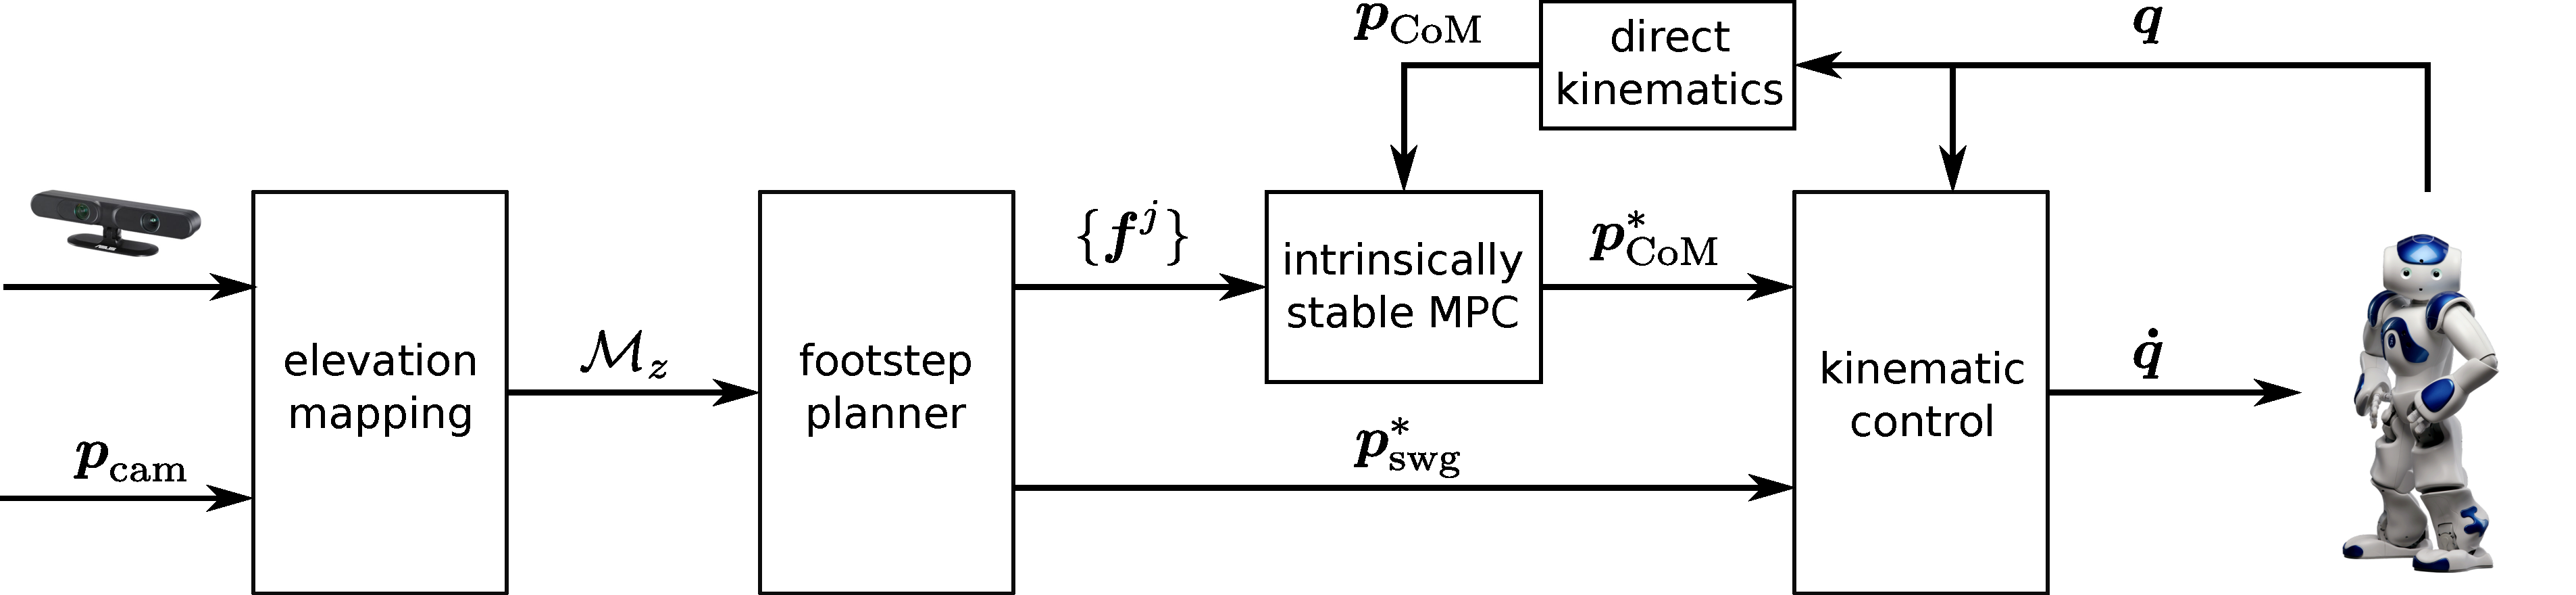
\includegraphics[width=\textwidth]{figures/BlockScheme.pdf}
    \caption{Block scheme of the approach.}
    \label{fig:block-scheme}
  \end{figure}
\end{frame}

\begin{frame}{Variable Height CoM IS-MPC: 3D Motion Model}
  \begin{columns}[c,onlytextwidth]
	  \column{0.7\textwidth}
      \begin{itemize}
        \item \textbf{LIP} model not suitable for gait generation over
						\textbf{uneven terrain}
				\item constraint vertical motion such that
			    \begin{equation*}
            \frac{\ddot{z}_c + g}{z_c - z_z} = \omega^2
          \end{equation*}
				\item CoM dynamics become
				  \begin{align*}
					  \ddot{x}_c &= \omega^2 (x_c - x_z)\\
					  \ddot{y}_c &= \omega^2 (y_c - y_z)\\
					  \ddot{z}_c &= \omega^2 (z_c - z_z) - g
				  \end{align*}
			\end{itemize}
		\column{0.3\textwidth}
		  \begin{figure}
        \centering
        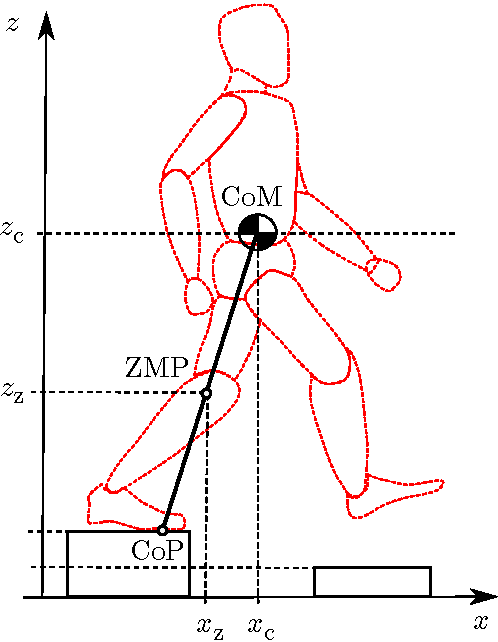
\includegraphics[width=\textwidth]{figures/LIPM_robot.pdf}
        \caption{ZMP, CoP and COM are colinear.}
        \label{fig:lipm-robot}
    \end{figure}
	\end{columns}
\end{frame}

\begin{frame}{Variable Height CoM IS-MPC: MPC Formulation}
  \begin{columns}[c,onlytextwidth]
	  \column{0.65\textwidth}
			\begin{itemize}
			  \item \textbf{constrain ZMP} into subregion of polyhedral cone (box)
					\begin{equation*}
%						-\frac{1}{2}
%						\begin{pmatrix}
%							\tilde{d}_x^\text{z} \\
%							\tilde{d}_y^\text{z} \\
%							d_z^\text{z}
%						\end{pmatrix}
%						\le
						R_{k+i}^T
						\begin{pmatrix}
							x_z^{k+i} - x_f^{k+i} \\
							y_z^{k+i} - y_f^{k+i} \\
							z_z^{k+i} - y_f^{k+i}
						\end{pmatrix}
						\le
						\frac{1}{2}
						\begin{pmatrix}
							\tilde{d}_x^\text{z} \\
							\tilde{d}_y^\text{z} \\
							d_z^\text{z}
						\end{pmatrix}
					\end{equation*}
				\item bound CoM wrt ZMP (\textbf{LIP stability})
					\begin{equation*}
						\frac{1}{\omega}\frac{1-e^{-\delta\omega}}{1-e^{-N\delta\omega}}
							\sum_{i=0}^{N-1} e^{-i\delta\omega} \dot{x}_z^{k+i} =
							x_c^k + \frac{\dot{x}_c^k}{\omega} - x_z^k
					\end{equation*}
			  \item solve \textbf{QP problem} using \textbf{MPC} scheme
			\end{itemize}
		\column{0.35\textwidth}
		  \begin{figure}
				\centering
				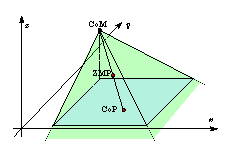
\includegraphics[width=\textwidth]{figures/balance3d.pdf}
				\caption{CoP internal to support polygon equivalent to ZMP internal
				    to polyhedral cone.}
				\label{fig:balance3d}
      \end{figure}
	\end{columns}
\end{frame}

\begin{frame}{Variable Height CoM IS-MPC: Stair Climbing}
	\begin{figure}
		\begin{subfigure}{0.40\textwidth}
			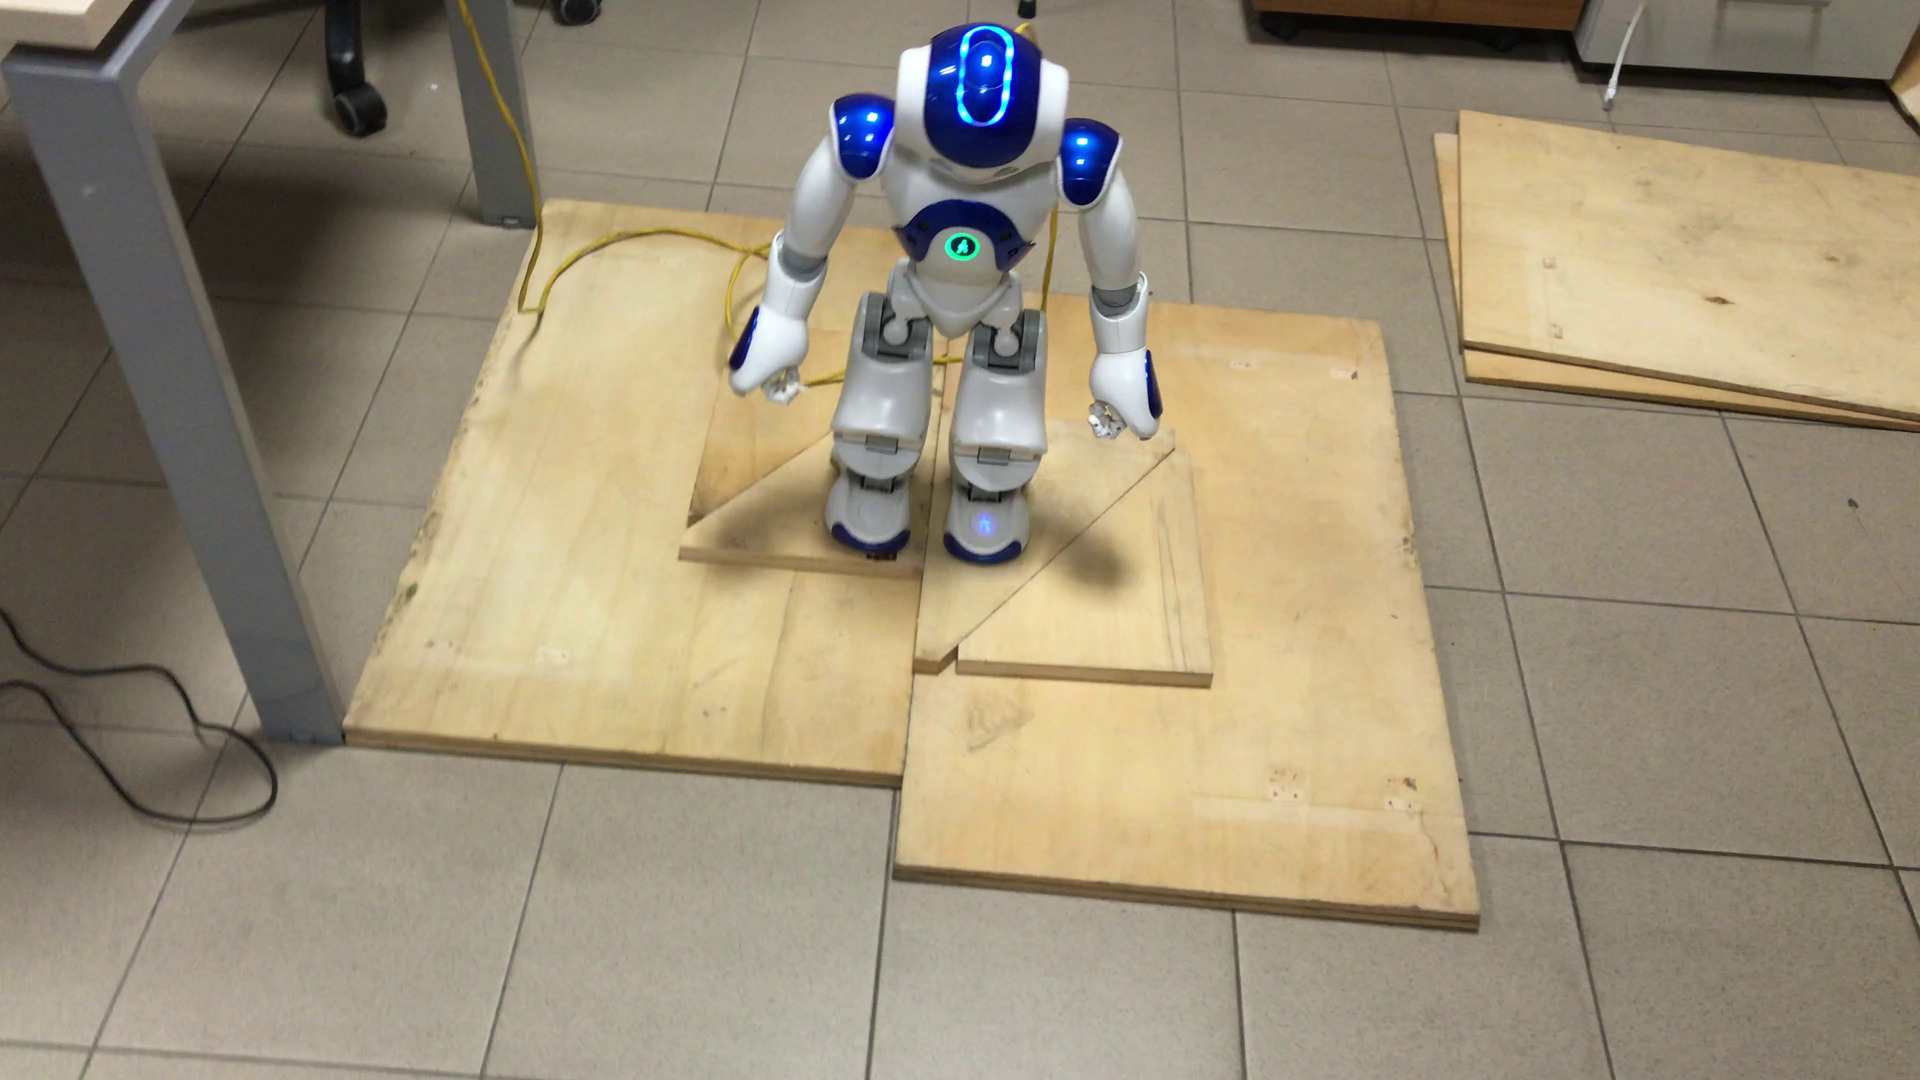
\includegraphics[width=\linewidth]
				{figures/experiments/multiple-staircases/downstairs/video/01.jpeg}
			%\caption{Starting position}
		\end{subfigure}\hspace*{0.05cm}%{\fill}
		\begin{subfigure}{0.40\textwidth}
			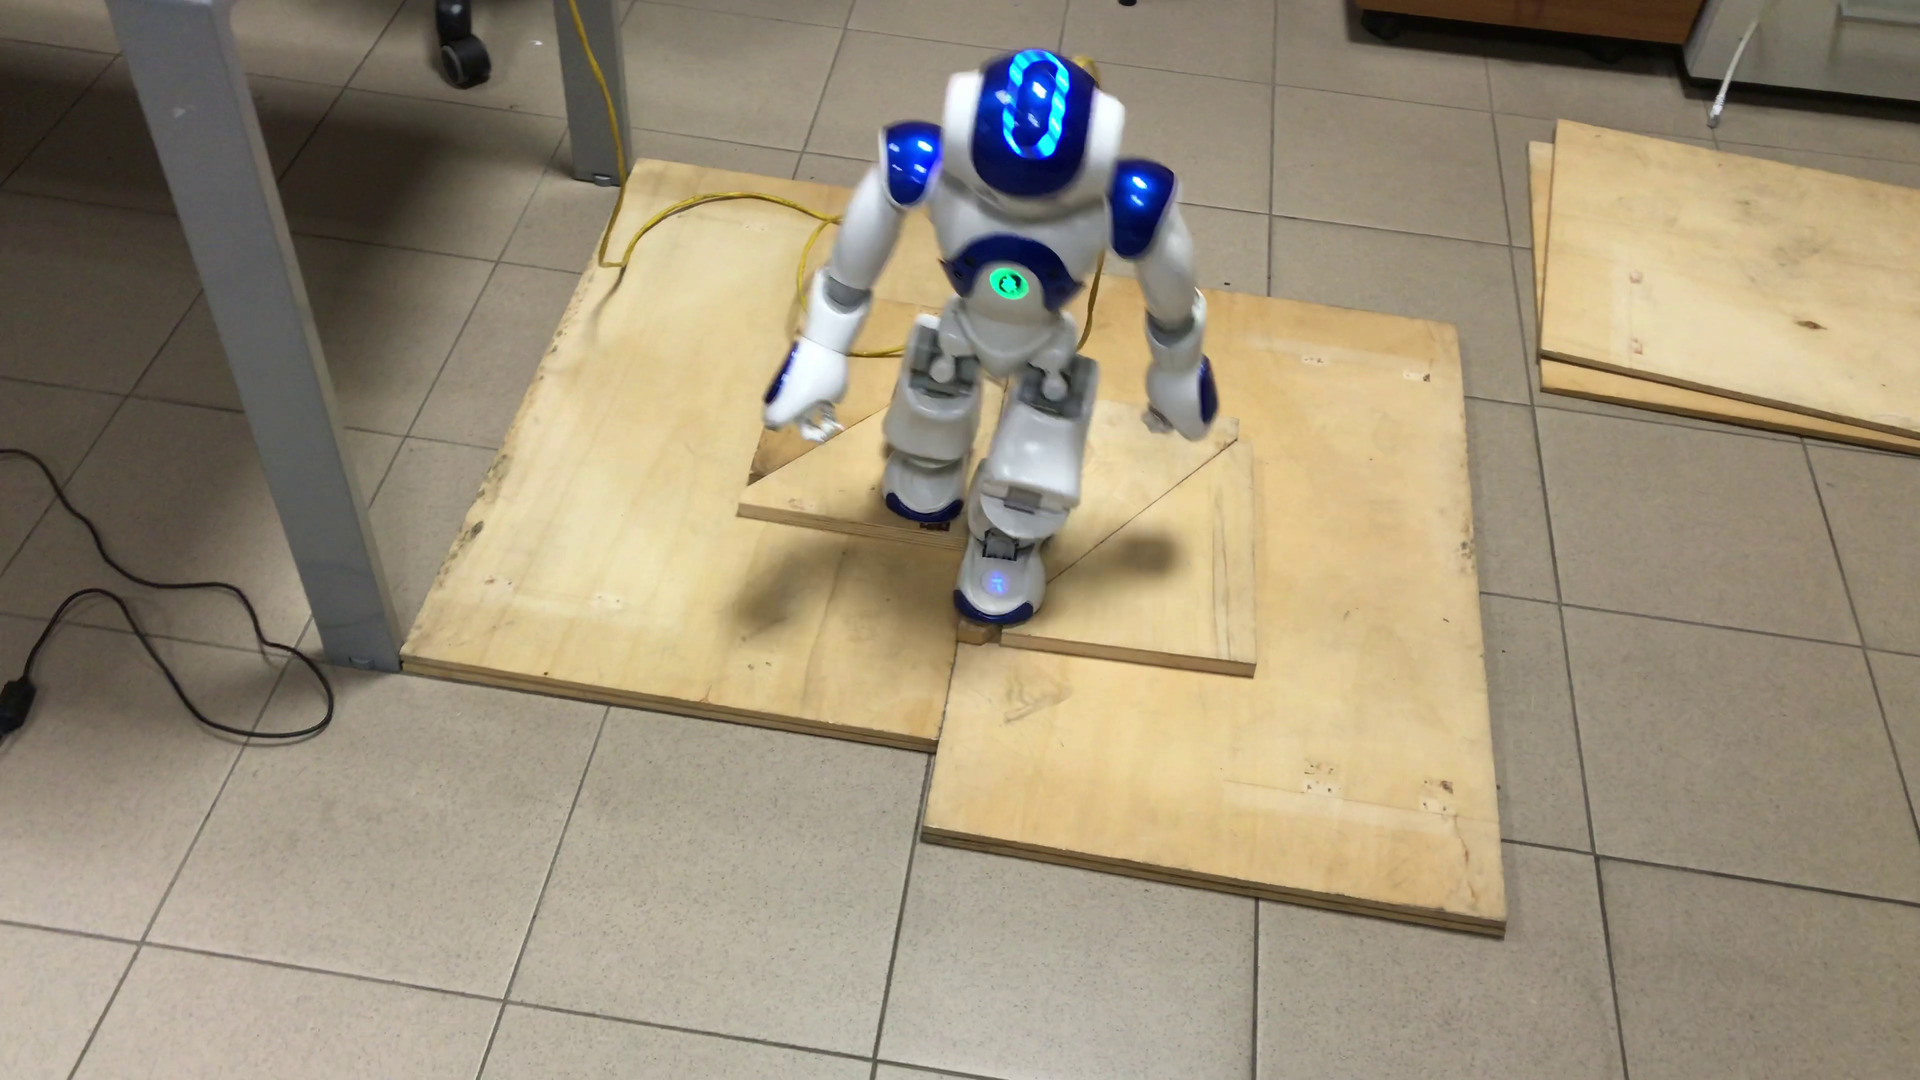
\includegraphics[width=\linewidth]
				{figures/experiments/multiple-staircases/downstairs/video/02.jpeg}
			%\caption{First step}
		\end{subfigure}
		\begin{subfigure}{0.40\textwidth}
			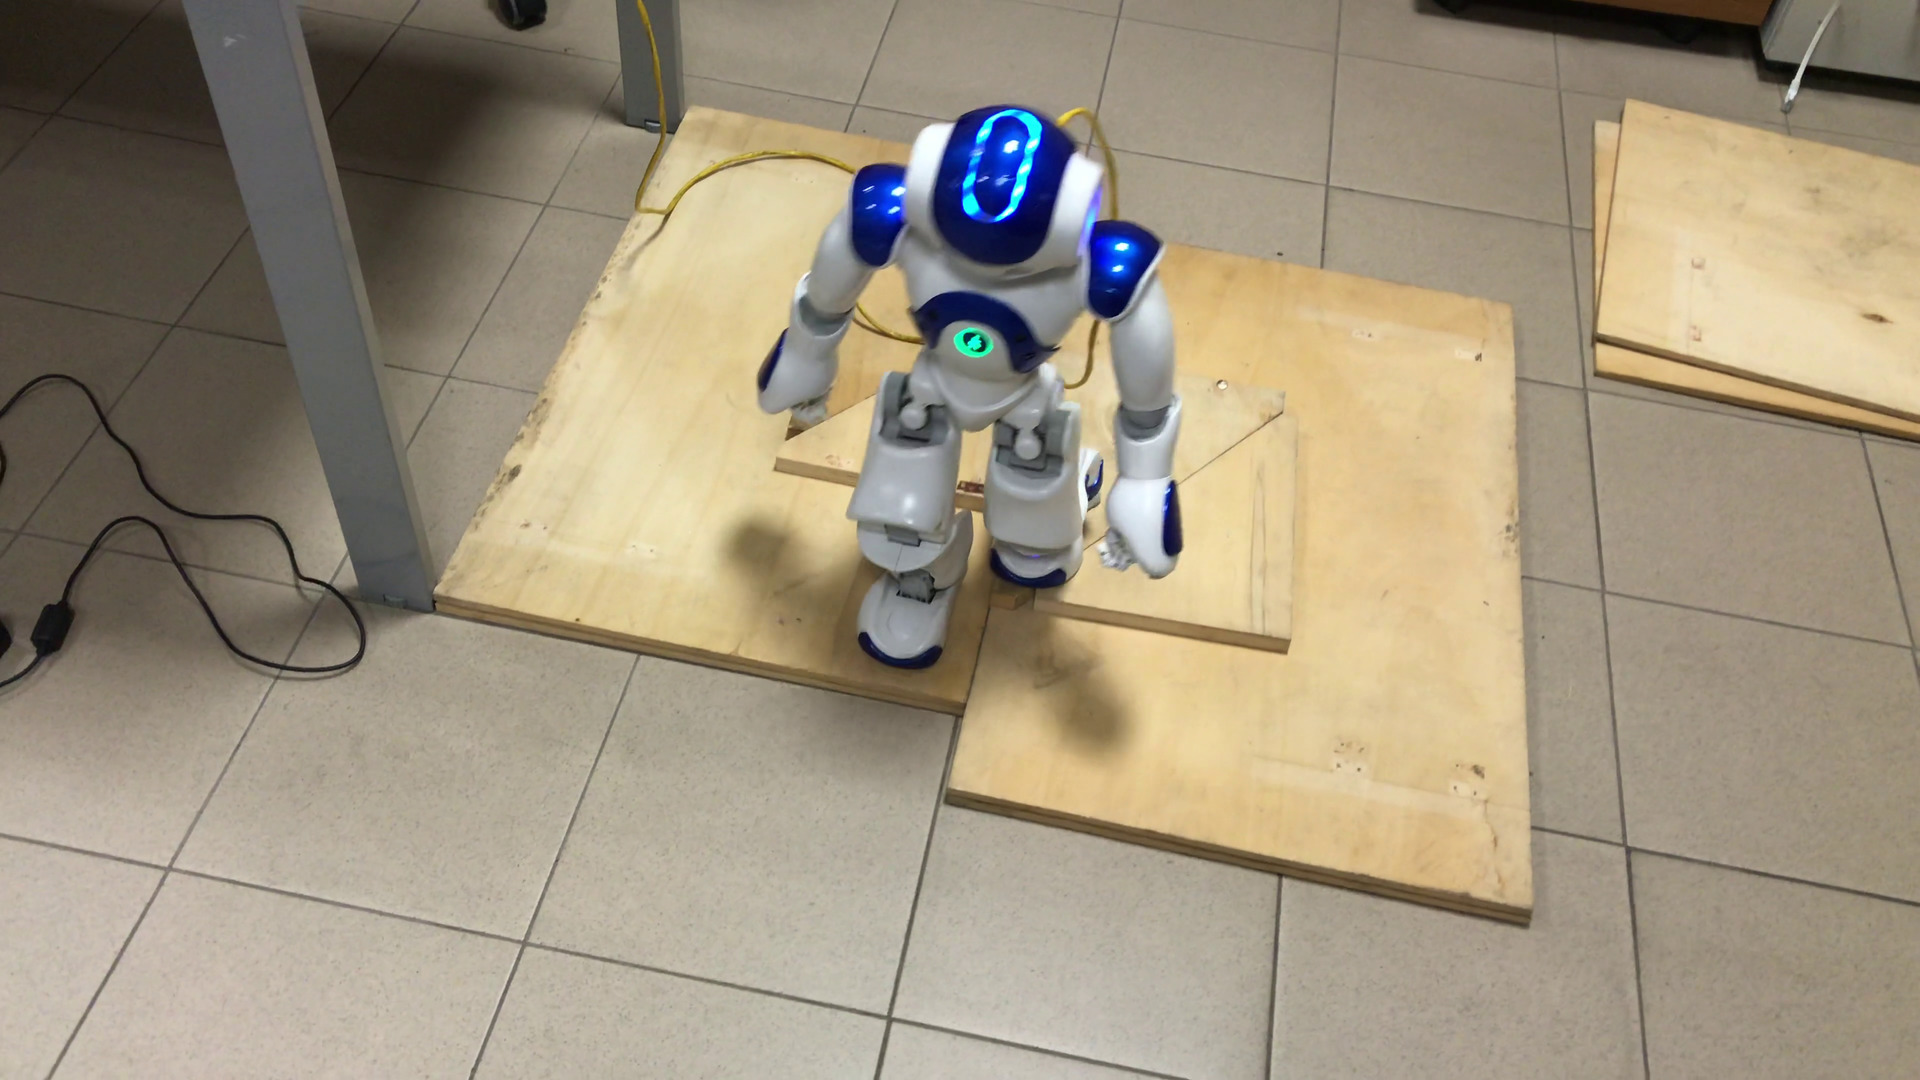
\includegraphics[width=\linewidth]
				{figures/experiments/multiple-staircases/downstairs/video/03.jpeg}
			%\caption{Second step}
		\end{subfigure}\hspace*{0.05cm}%{\fill}
		\begin{subfigure}{0.40\textwidth}
			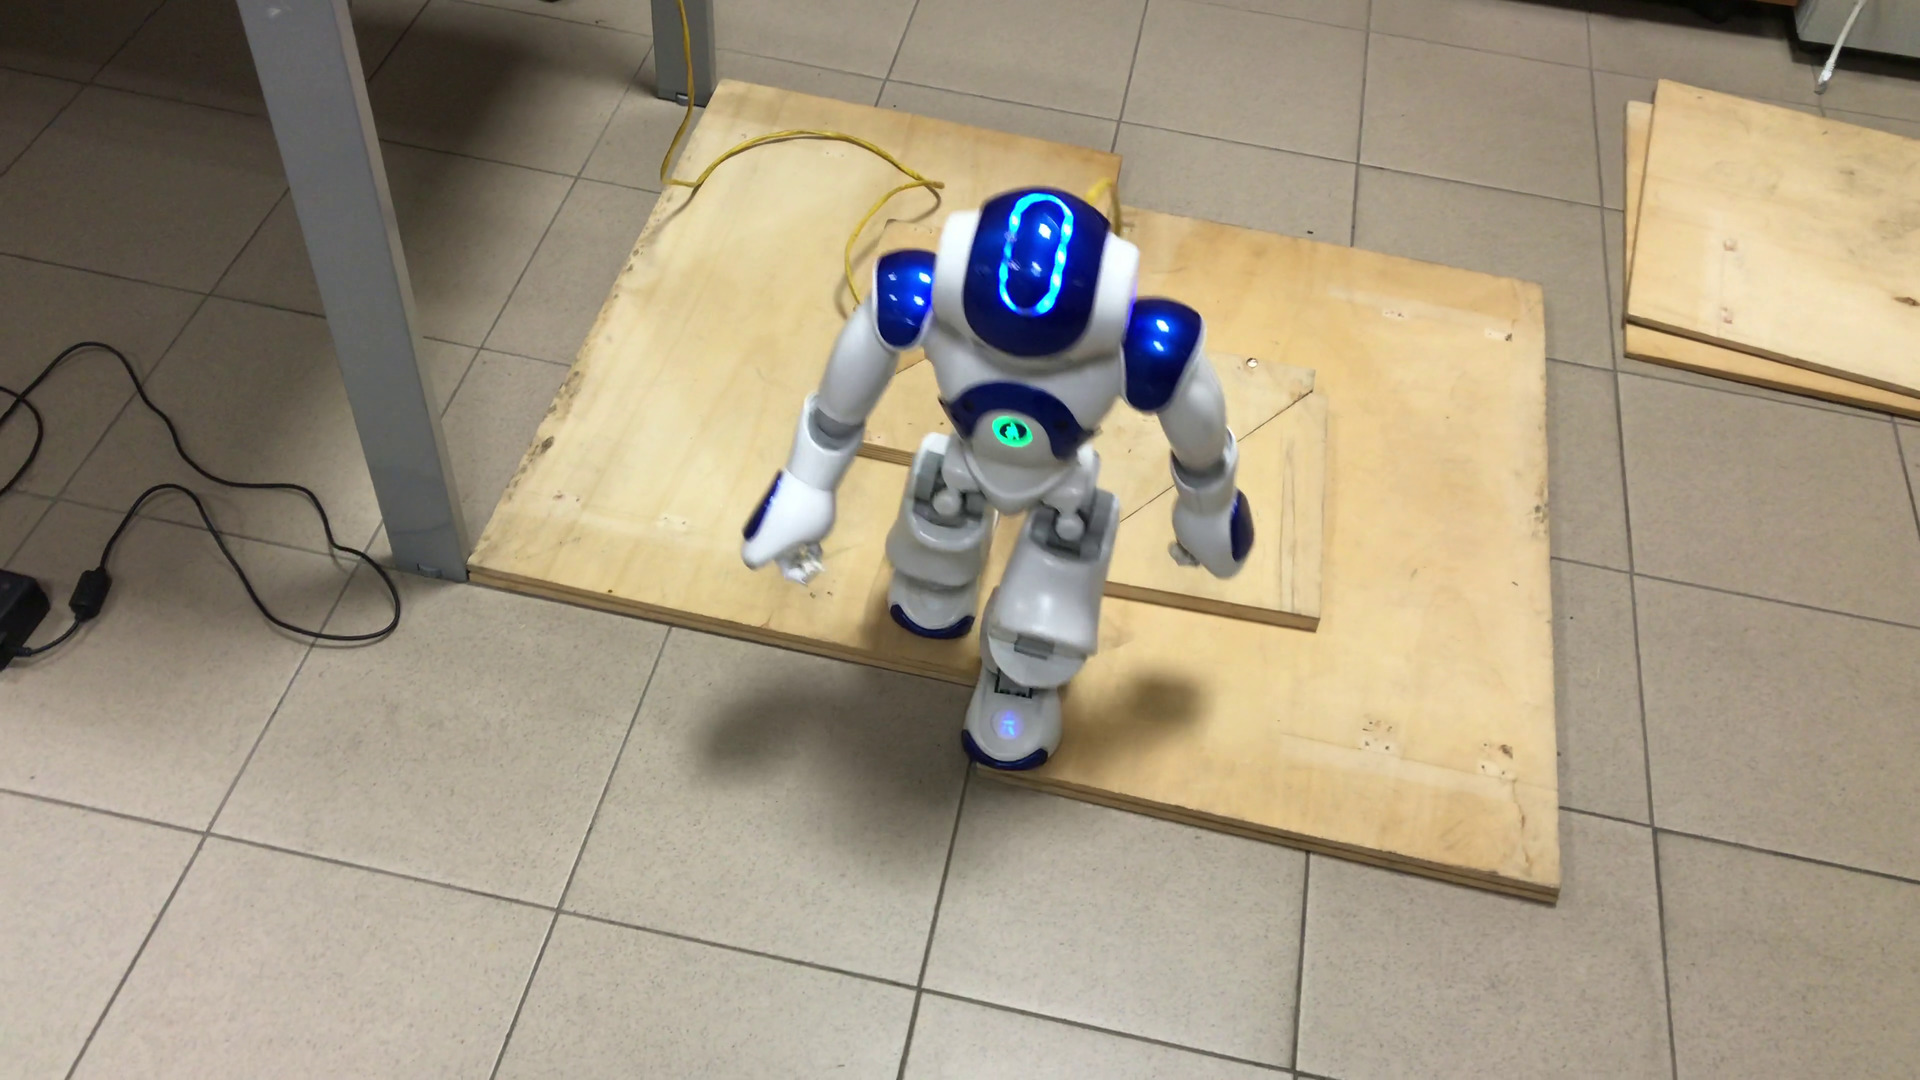
\includegraphics[width=\linewidth]
				{figures/experiments/multiple-staircases/downstairs/video/04.jpeg}
			%\caption{Third step}
		\end{subfigure}
		\begin{subfigure}{0.40\textwidth}
			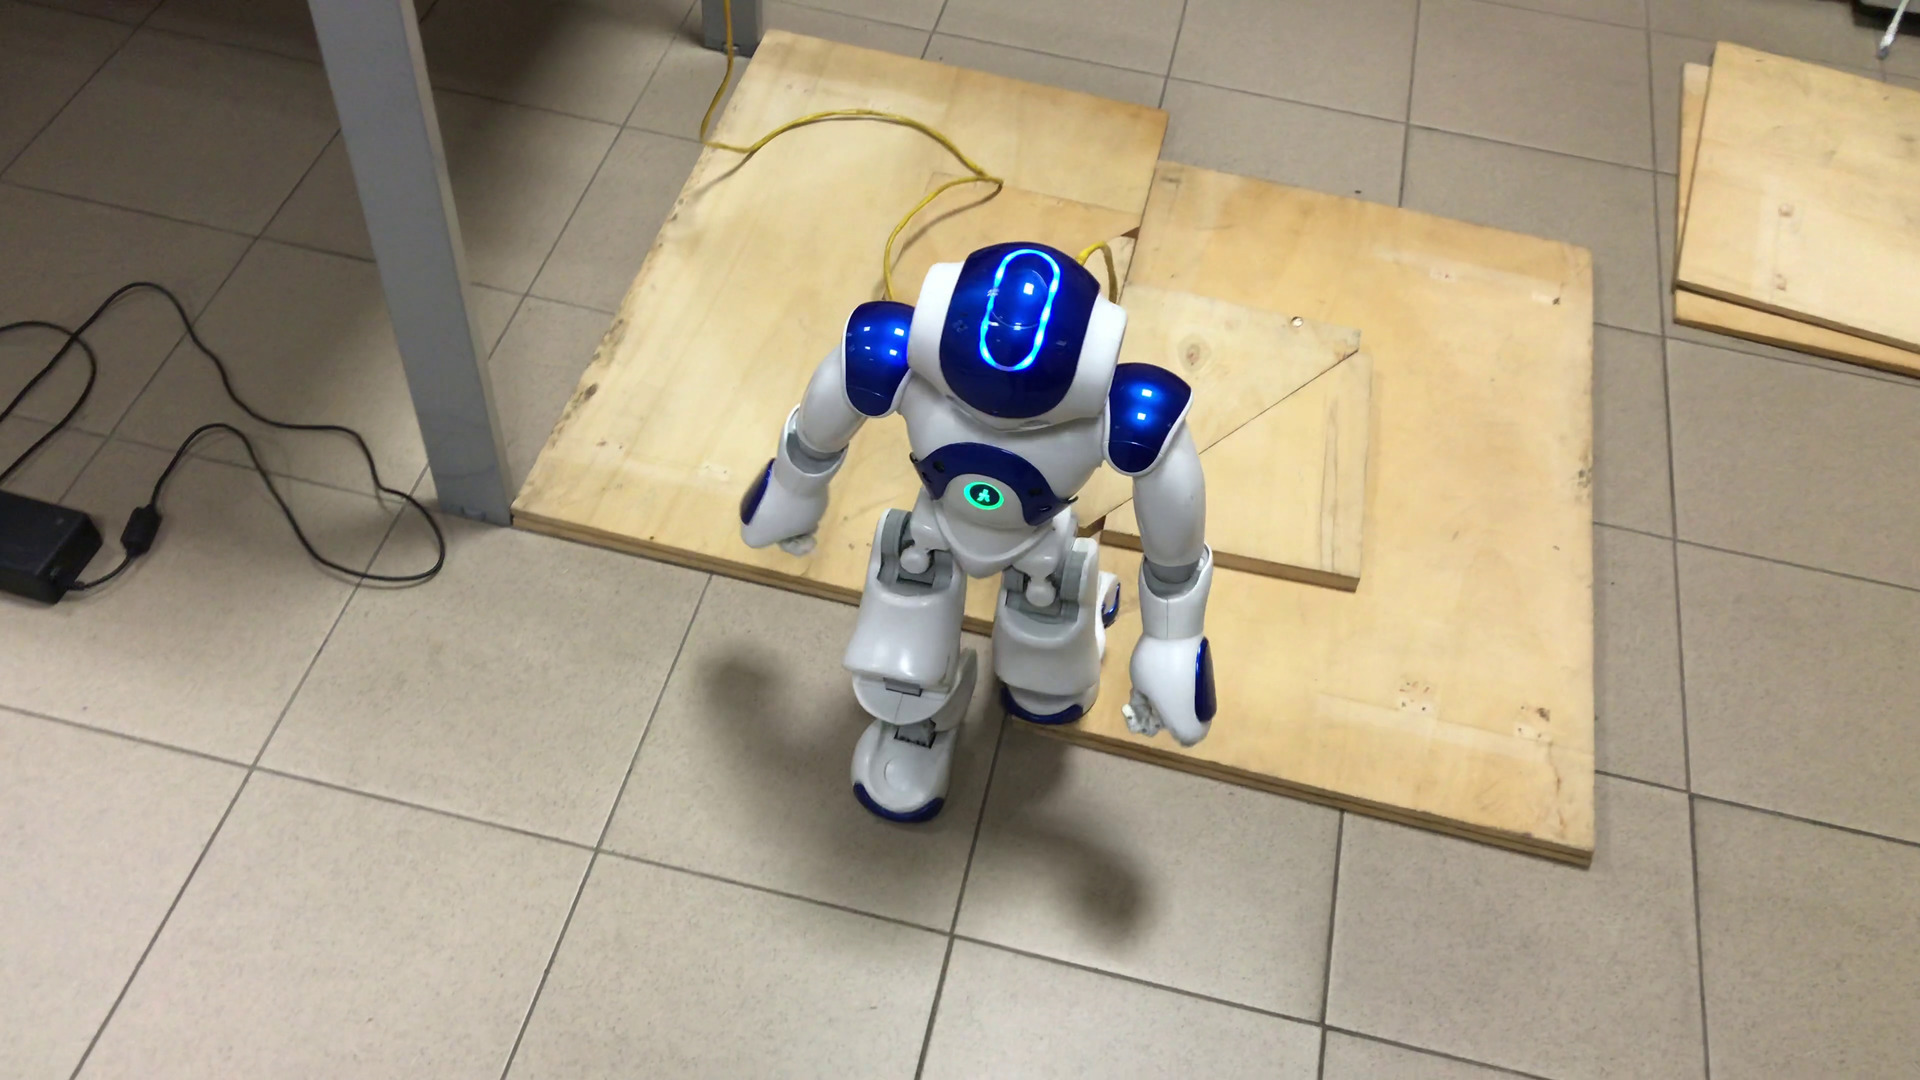
\includegraphics[width=\linewidth]
				{figures/experiments/multiple-staircases/downstairs/video/05.jpeg}
			%\caption{Fourth step}
		\end{subfigure}\hspace*{0.05cm}%{\fill}
		\begin{subfigure}{0.40\textwidth}
			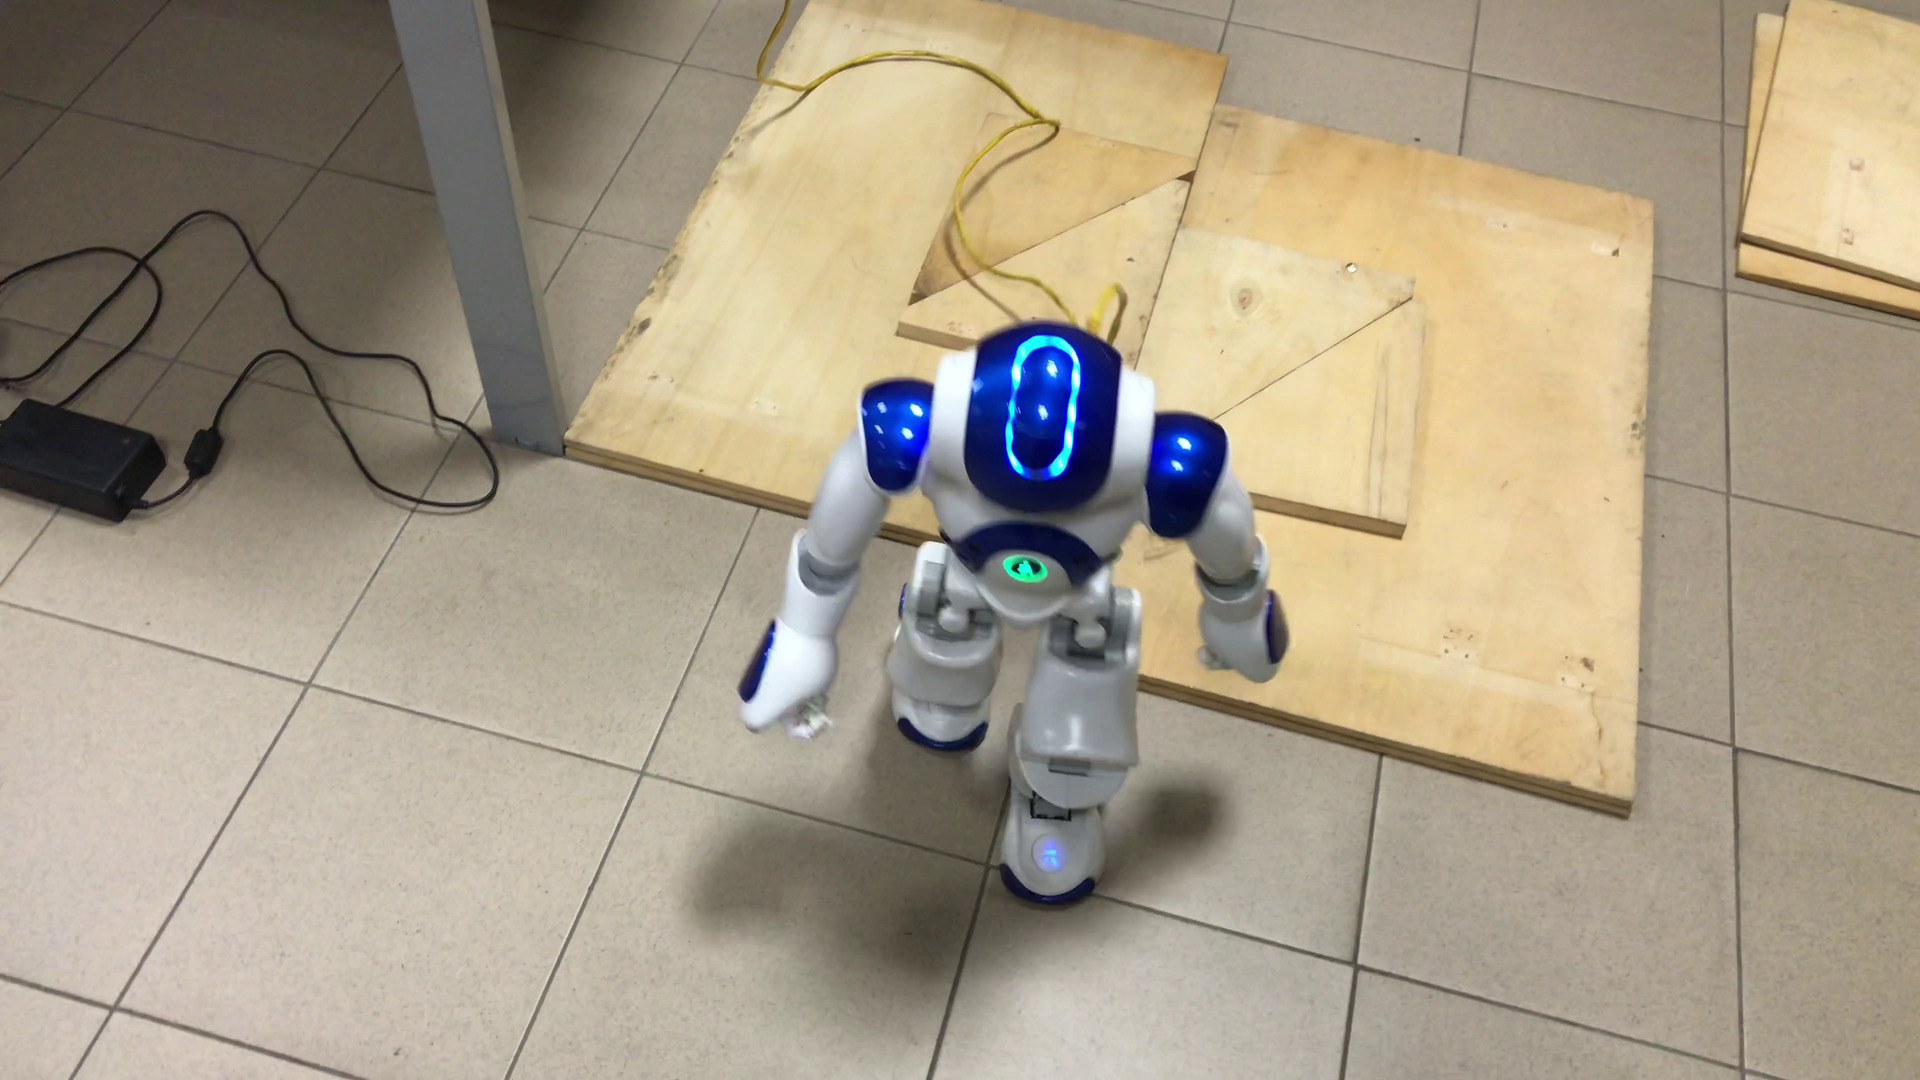
\includegraphics[width=\linewidth]
				{figures/experiments/multiple-staircases/downstairs/video/06.jpeg}
			%\caption{Fifth step}
		\end{subfigure}
		\caption{NAO going down the stairs.}
		%\caption{The figures show the motion of the robot for the scenario
		%		``Multiple Staircases (Downstairs)''. The robot starts on top of the 
		%		stairway (Fig. \ref{fig:exp:ms:down:frame1}), then it places 
		%		each step one in front of the other without colliding with the staircases,
		%		safely reaching ground level. Each staircase has a height of 2 cm.}
	\end{figure}
\end{frame}

\begin{frame}{Variable Height CoM IS-MPC: Stair Climbing}	
	\begin{figure}
		\centering
		%\includegraphics[width=0.5\textwidth]
		%		{figures/experiments/multiple-staircases/downstairs/xy-plot-2cm.pdf}
		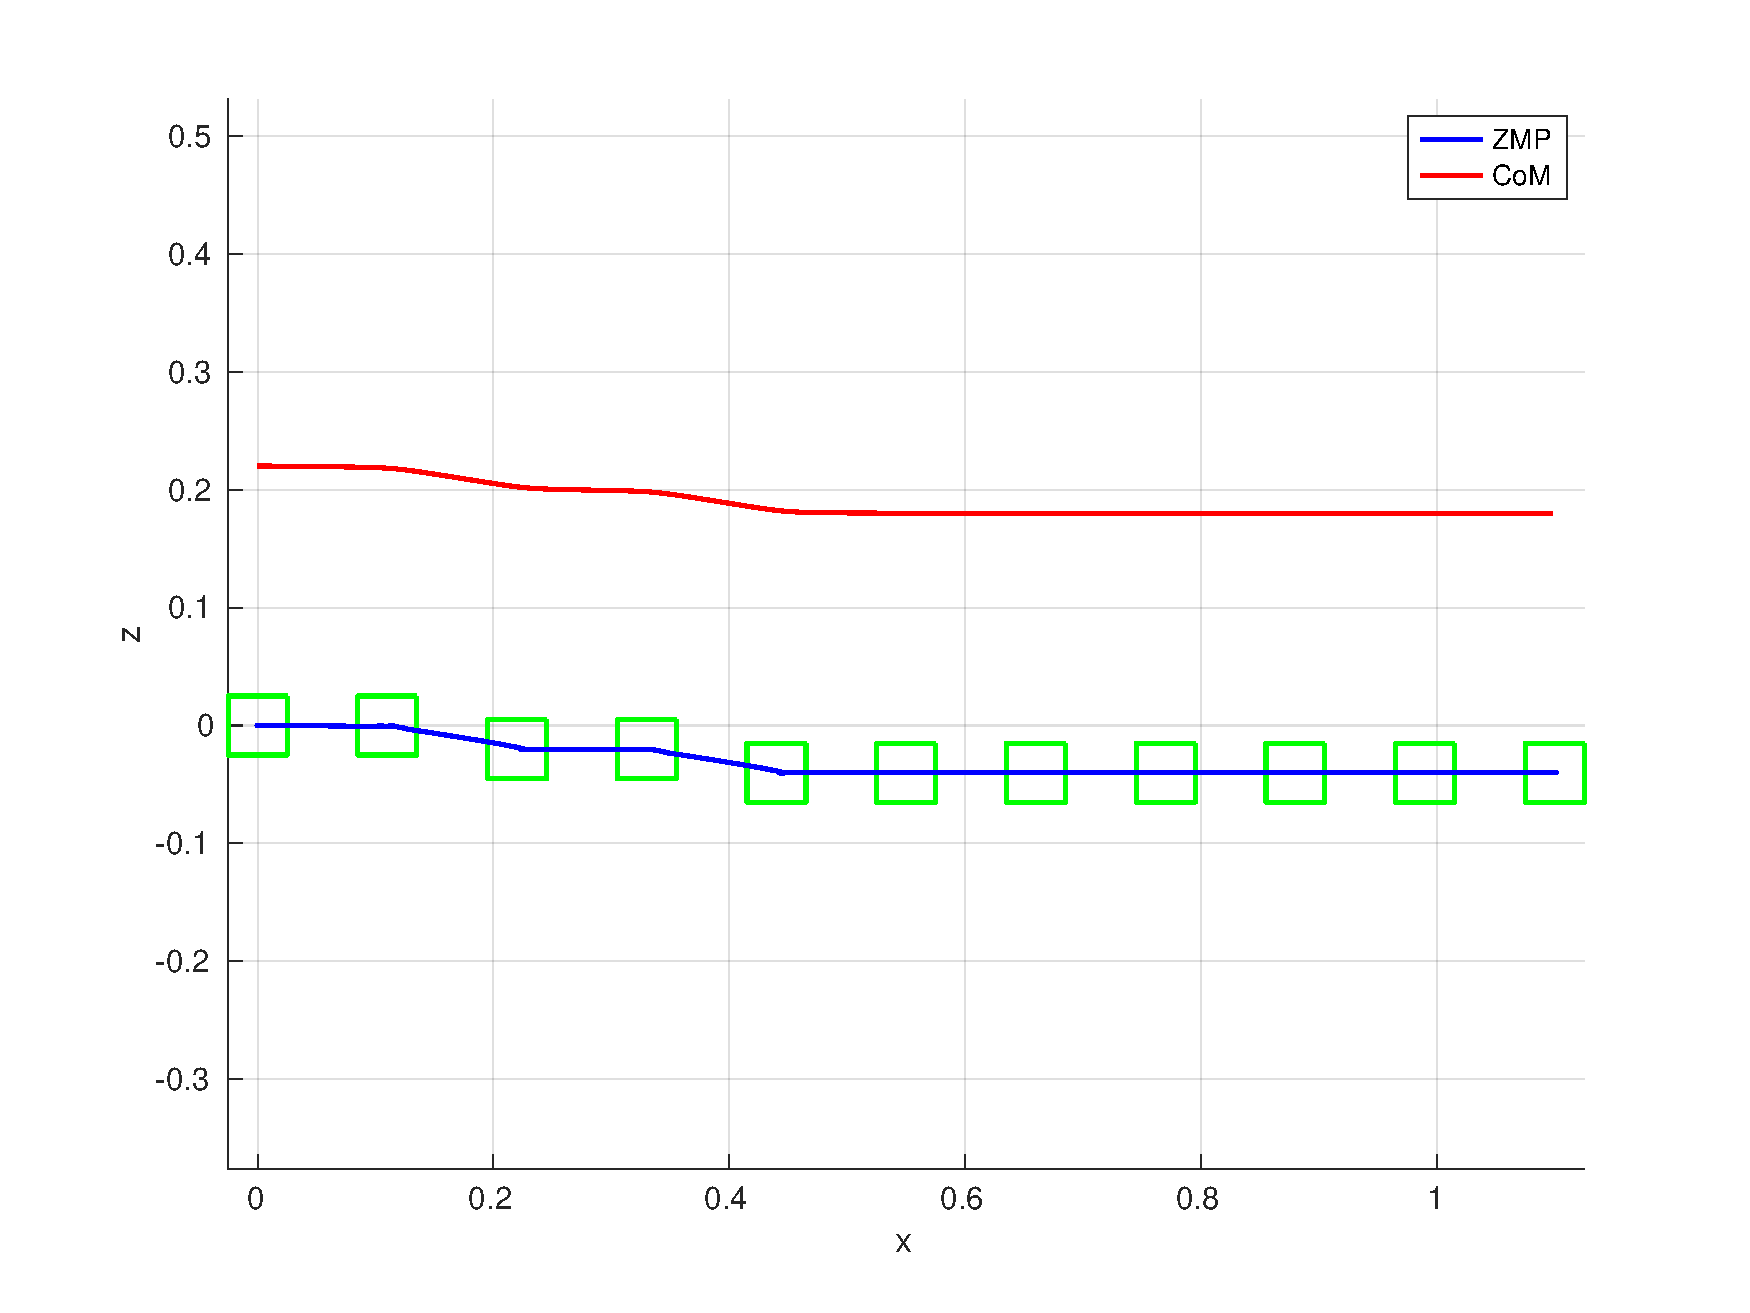
\includegraphics[width=0.8\textwidth]
				{figures/experiments/multiple-staircases/downstairs/xz-plot-2cm.pdf}
		\caption{CoM/ZMP plot ($z$-axis).}
		%\caption{The plots show how the CoM and the ZMP vary with respect to the
		%	footsteps in the scenario ``Multiple Staircases (Downstairs)''.
		%	The green boxes represent the footsteps.}
	\end{figure}
\end{frame}

\begin{frame}{RRT-based Footstep Planning}
  \begin{itemize}
    \item \textbf{Rapidly-Exploring Random Tree}
			\begin{itemize}
        \item[R1] maximum footsteps height variation
				    $|z_{\rm f}^j - z_{\rm f}^{j-1}| \le \Delta z_{\max}$
        \item[R2] footstep is fully in contact with the ground
        \item[R3] swing foot trajectory $\bfp_{\rm {swg}}^j$ is collision free
			\end{itemize}
    \item footstep planner iteration
			\begin{enumerate}
        \item $\bfp_{\rm rand} \leftarrow {\text Rand}(\mathcal{M}_z)$
				\item $v_{\rm near} \leftarrow Nearest(\bfp_{\rm rand}, \gamma,
            \mathcal{T})$
        \item $\bff_{\rm cand} \leftarrow {\text Rand}(U)$
				\item \textbf{if} $\bff_{\rm cand}$ feasible wrt R1-R2 \textbf{then}
				\item $\quad$ $\bfp_{\rm swg}^{\rm cand}
						\leftarrow \text{BuildTrajectory}(\cdot)$
				\item $\quad$ $\mathcal{T}\text{.add}(v_{\rm new}, v_{\rm near})$
						\textbf{if} $\bfp_{\rm swg}^{\rm cand}$ satisfies R3
      \end{enumerate}
	\end{itemize}
\end{frame}

\begin{frame}{RRT-based Footstep Planning: Catalogue of Primitives}
	\begin{figure}
			\centering
			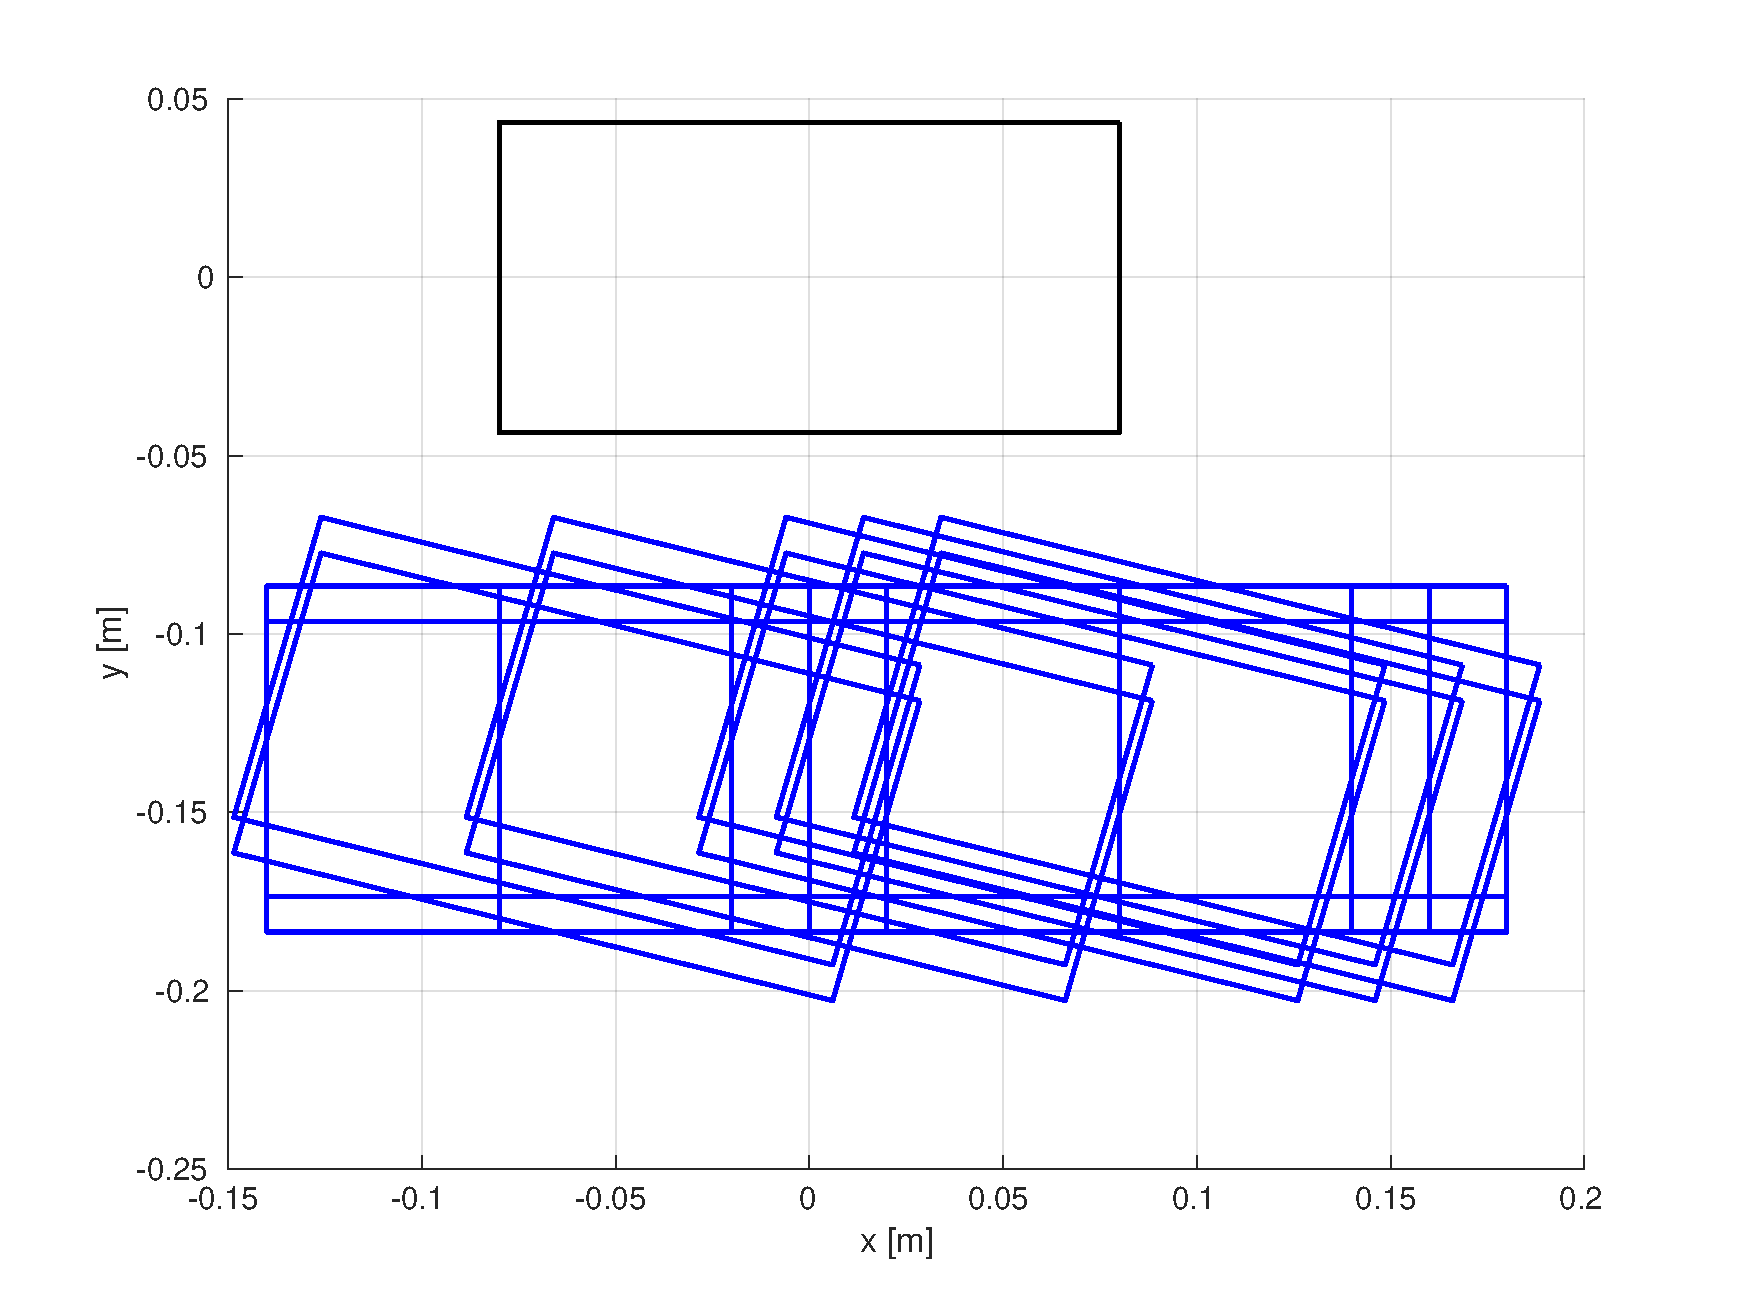
\includegraphics[width=0.8\textwidth]{figures/catalogue-primitives.pdf}
			\caption{NAO's catalogue of primitives $U$.}
% The catalogue of primitives (blue color) specifies the possible
% poses of the
% candidate footstep $\bff^{\rm cand}$ with respect to the pose of the 
% current support foot $\bff_{\rm sup}^{\rm near}$. The figure shows the 
% case where the left foot is the support foot. The catalogue for the 
% case where the right foot is the support foot is specular. The $z$
% coordinate of a candidate footstep can be retrieved directly from 
% the elevation map $\mathcal{M}_z$.}
	\end{figure}
\end{frame}

\begin{frame}{RRT-based Footstep Planning: Obstacle Avoidance}
	\begin{figure}
		\begin{subfigure}{0.40\textwidth}
			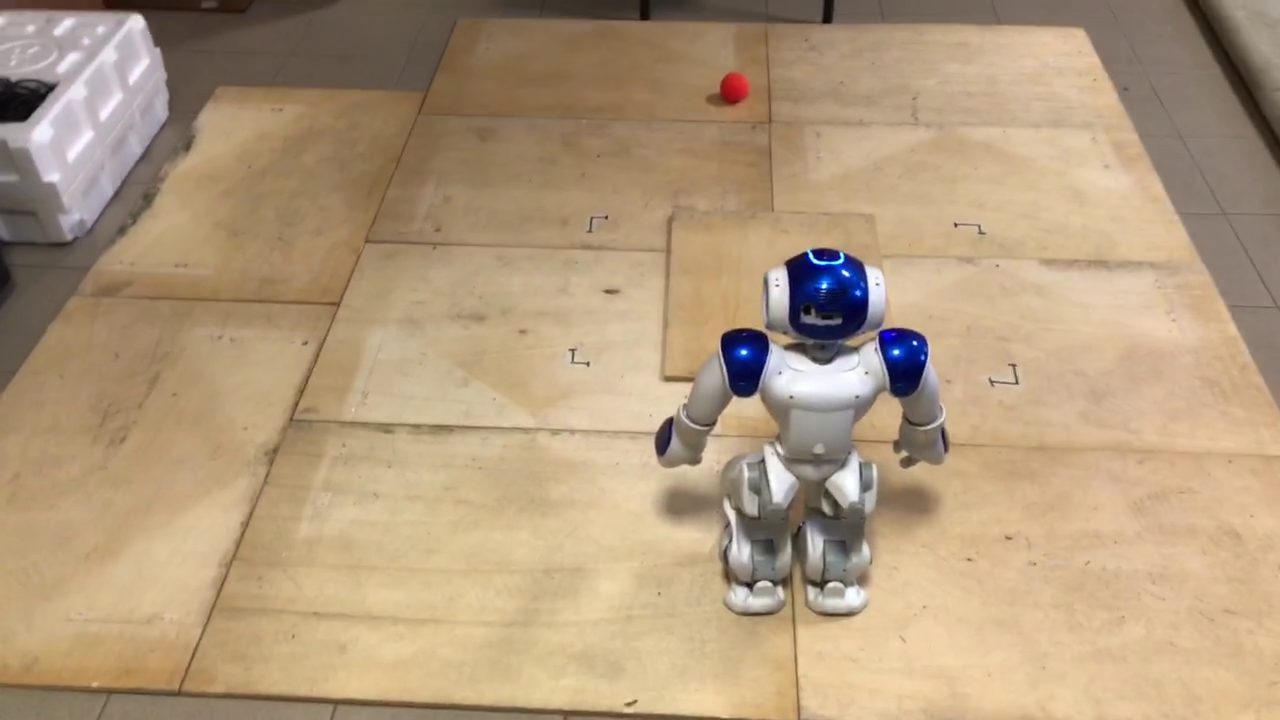
\includegraphics[width=\linewidth]
				{figures/experiments/obstacle-avoidance/video/01.png}
			%\caption{Starting position}
		\end{subfigure}\hspace{0.05cm}%*{\fill}
		\begin{subfigure}{0.40\textwidth}
			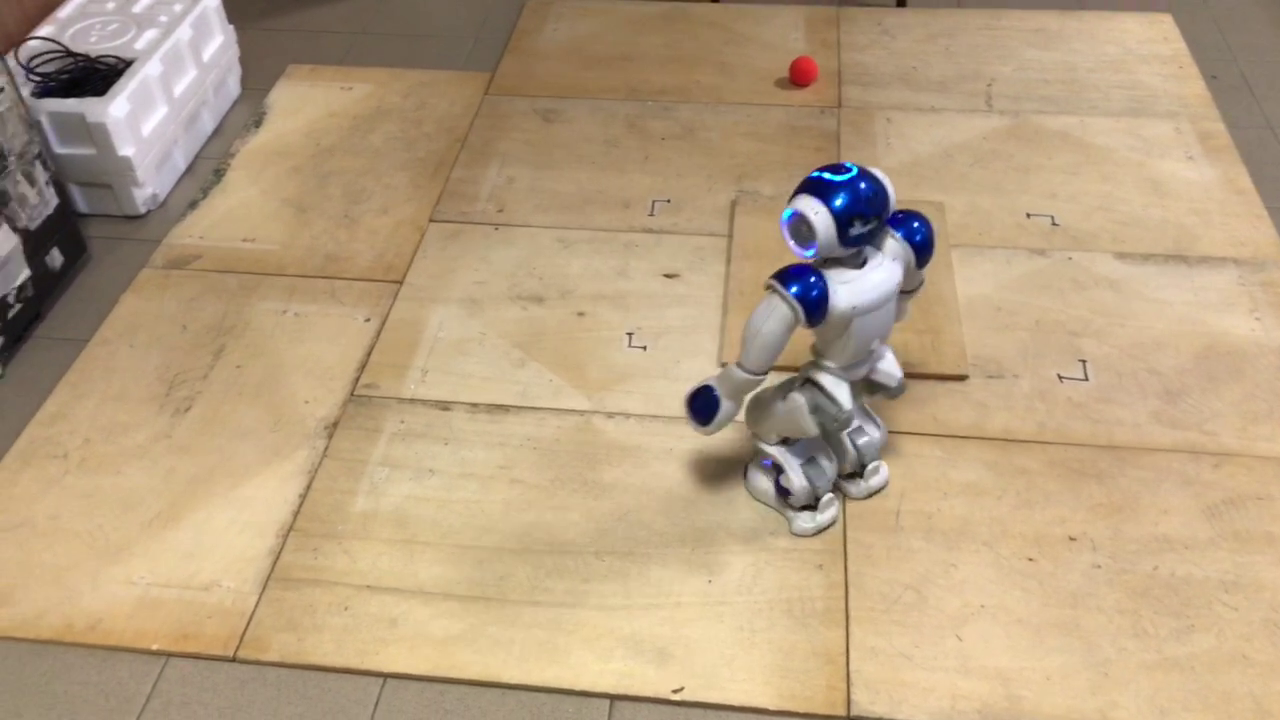
\includegraphics[width=\linewidth]
				{figures/experiments/obstacle-avoidance/video/02.png}
			%\caption{Moving to the left}
		\end{subfigure}
		\begin{subfigure}{0.40\textwidth}
			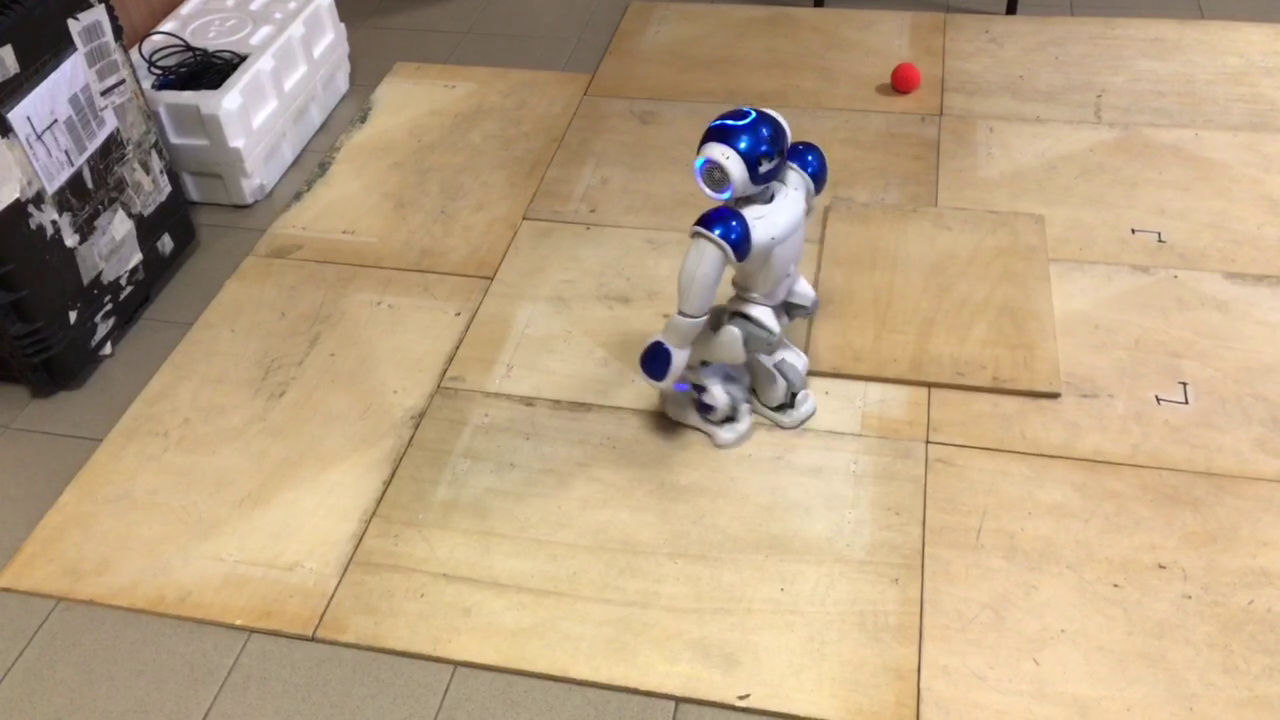
\includegraphics[width=\linewidth]
				{figures/experiments/obstacle-avoidance/video/03.png}
			%\caption{Avoiding the obstacle}
		\end{subfigure}\hspace{0.05cm}%*{\fill}
		\begin{subfigure}{0.40\textwidth}
			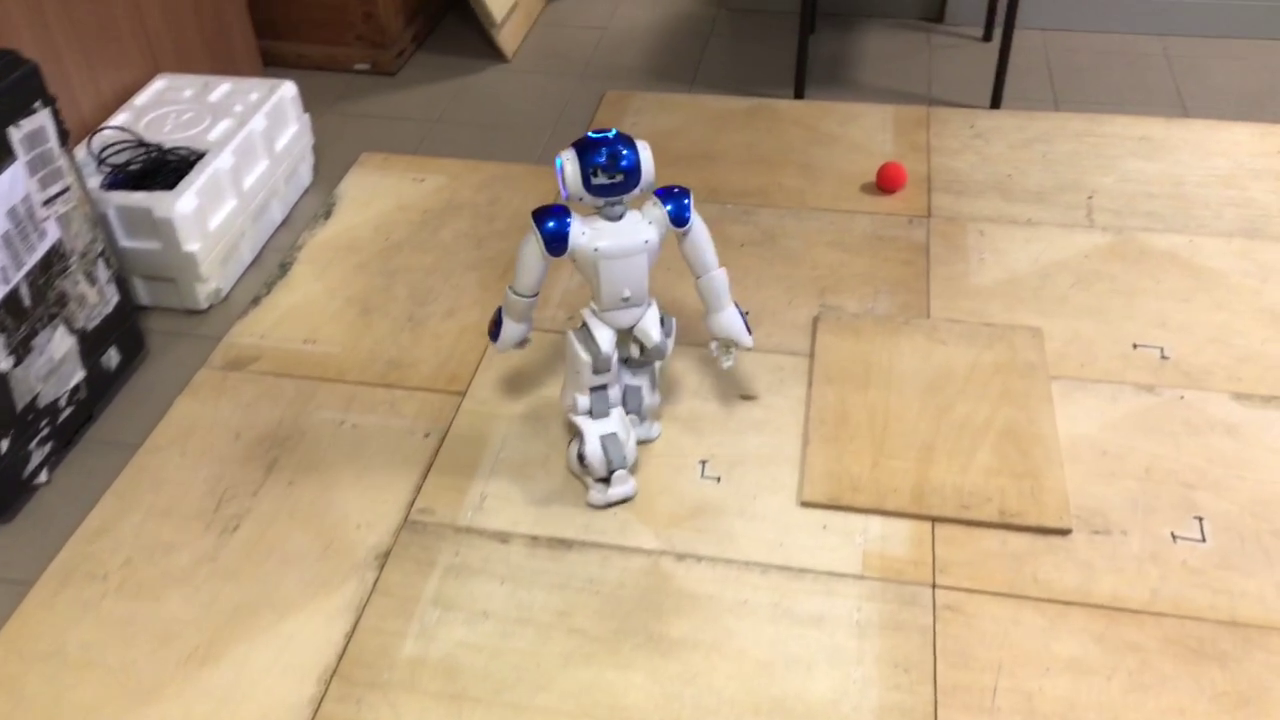
\includegraphics[width=\linewidth]
				{figures/experiments/obstacle-avoidance/video/04.png}
			%\caption{Moving forward}
		\end{subfigure}
		\begin{subfigure}{0.40\textwidth}
			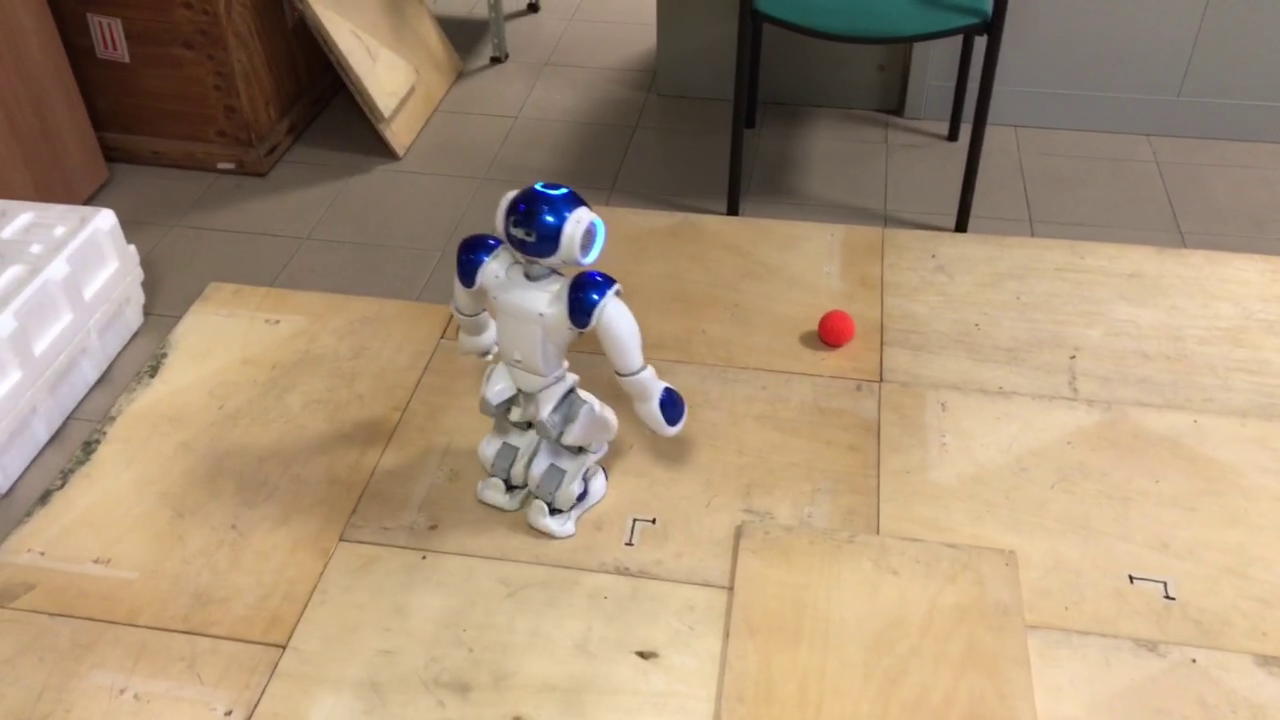
\includegraphics[width=\linewidth]
				{figures/experiments/obstacle-avoidance/video/05.png}
			%\caption{Moving towards the goal}
		\end{subfigure}\hspace{0.05cm}%*{\fill}
		\begin{subfigure}{0.40\textwidth}
			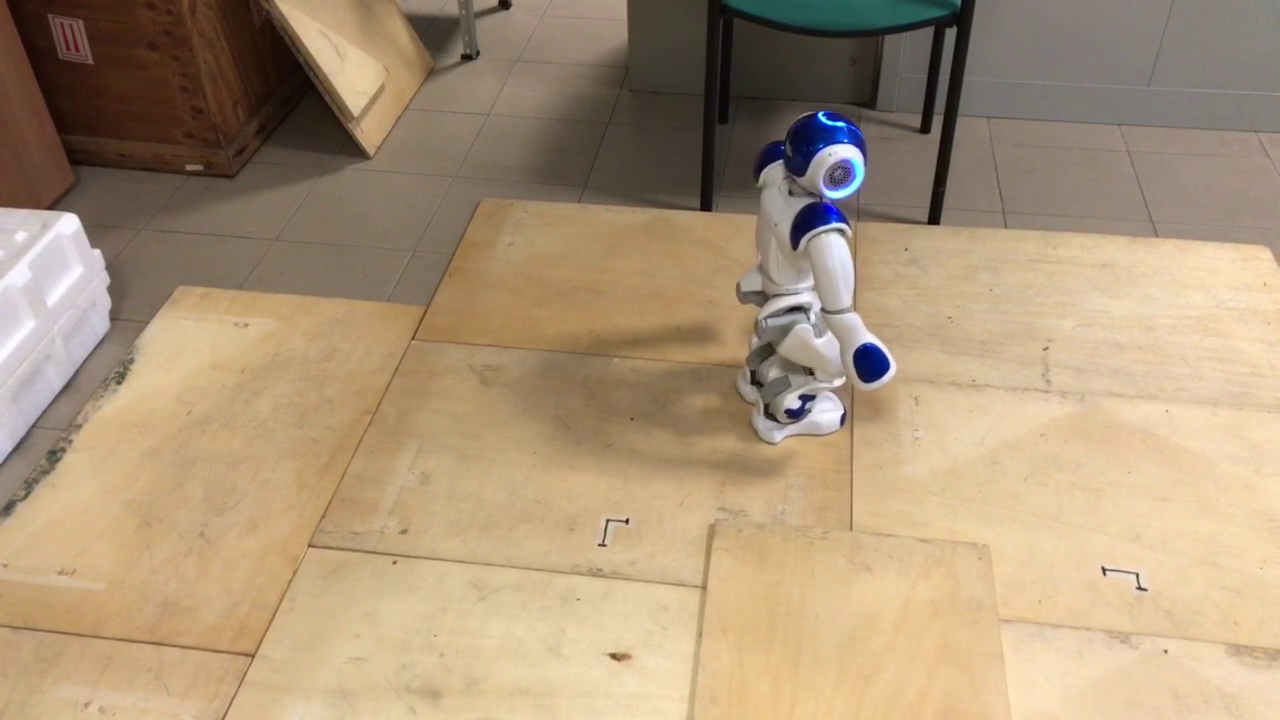
\includegraphics[width=\linewidth]
				{figures/experiments/obstacle-avoidance/video/06.png}
			%\caption{Goal region reached}
		\end{subfigure}
		\caption{NAO avoiding an obstacle.}
	\end{figure}
\end{frame}

\begin{frame}{RRT-based Footstep Planning: Obstacle Avoidance}
	\begin{center}
    tree size: 488 -- solution size: 31 -- runtime: 70 ms
  \end{center}
	\begin{figure}
		\centering
		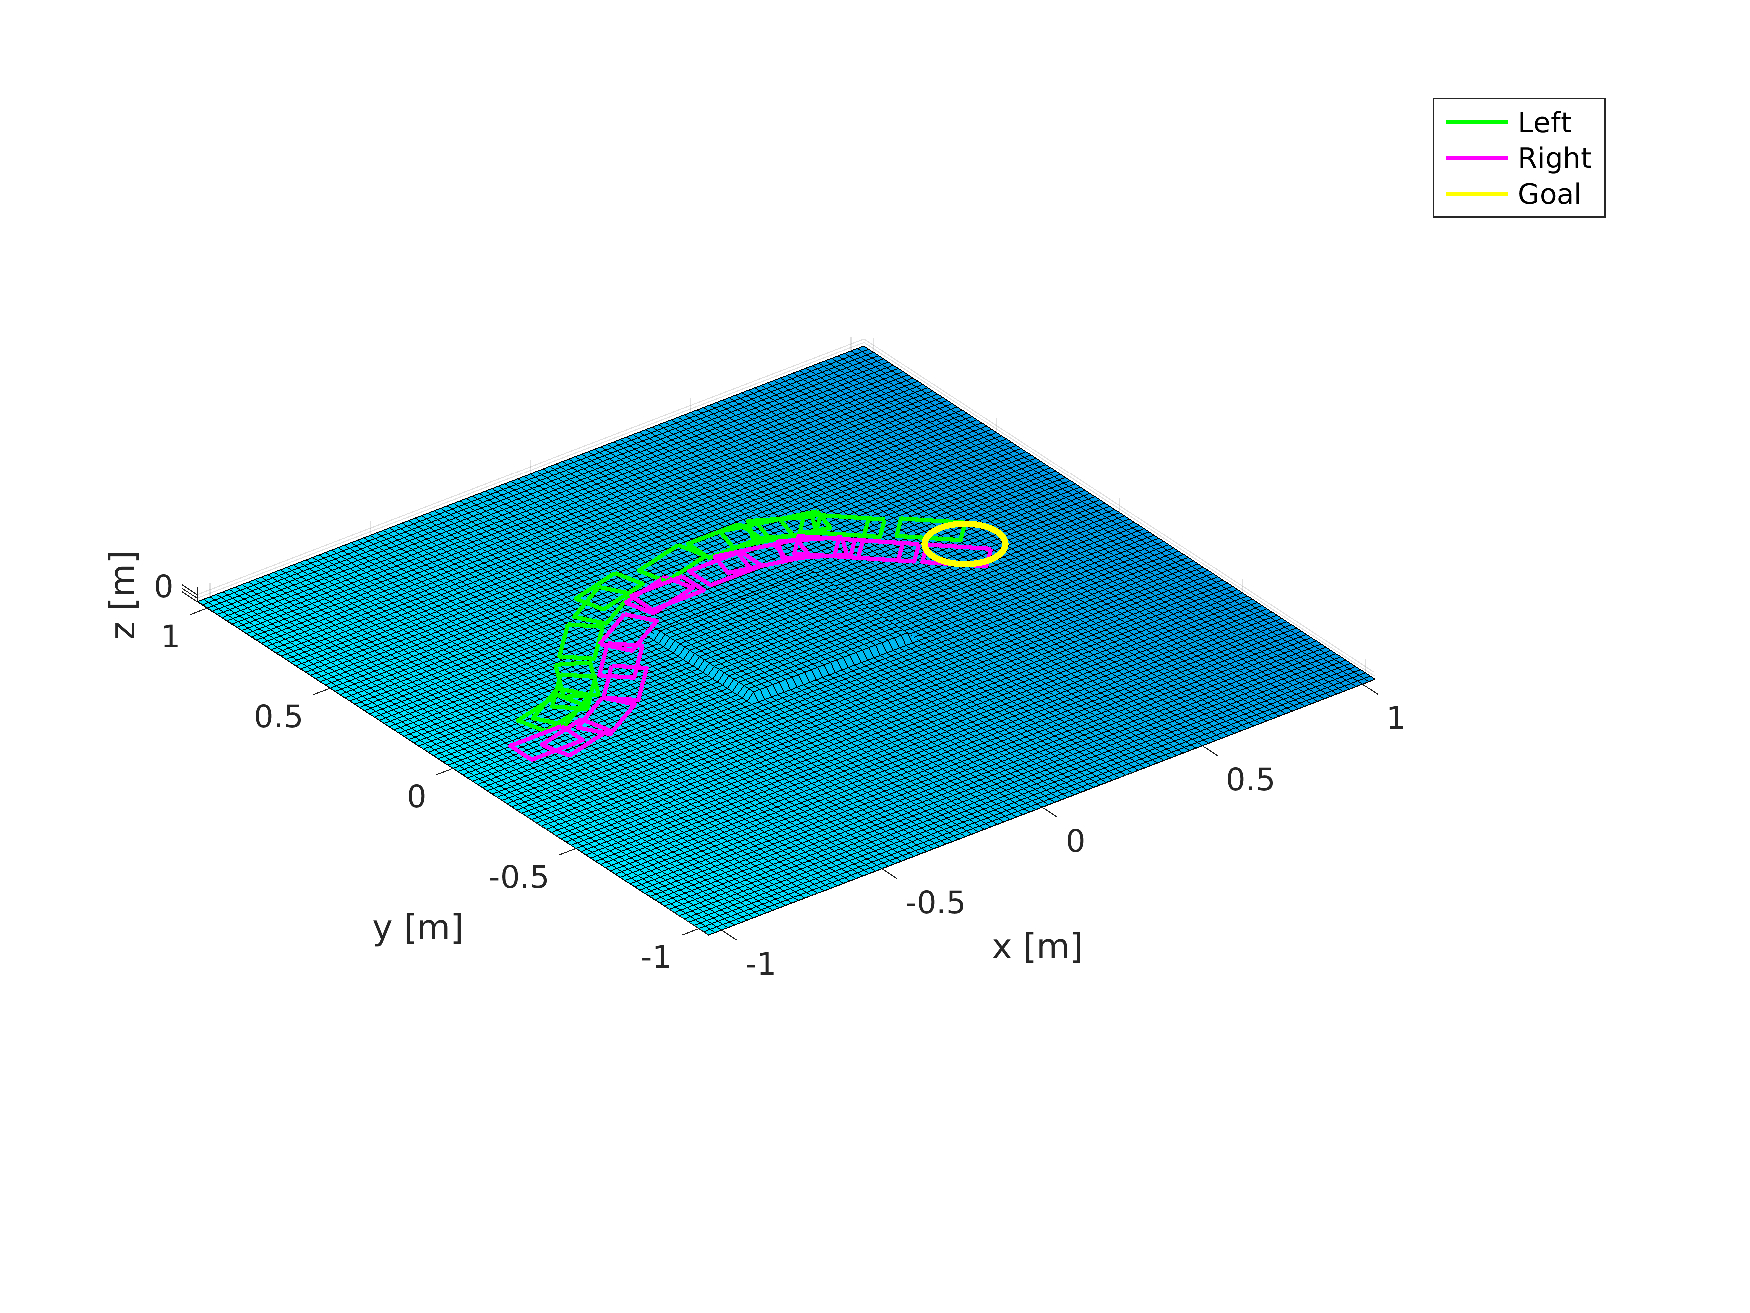
\includegraphics[width=0.8\textwidth]
				{figures/experiments/obstacle-avoidance/footstep-plan.pdf}
		\caption{Footstep plan generated for the scenario ``Obstacle Avoidance''.}
	\end{figure}
\end{frame}

\begin{frame}{Elevation Map Generation: Framework}
	\texttt{elevation\_mapping}
  \begin{itemize}
		\item robot-centric grid-based map: $\mathcal{M}_z$
		\item height estimate $\mathcal{N}(\hat{h}_i, \sigma_{h_i}^2)$
				for each cell $i$
		\item \textbf{Kalman filter} given new height and motion measurements
		\item \textbf{map fusion}: $(\hat{h}_i, h_{i,\min}, h_{i,\max})$ such that
				$h_i \in [h_{i,\min}, h_{i,\max}]$ with 95\% confidence
		\item \textbf{dynamic environments} using visibility check based
				on ray tracing
	\end{itemize}
\end{frame}

\begin{frame}{Elevation Map Generation: Settings}
	\begin{columns}[c,onlytextwidth]
		\column{0.65\textwidth}
			\begin{itemize}
				\item NAO humanoid robot
				\item ASUS Xtion Pro (\textbf{depth} sensor)
				\item working range: 0.5--3.5 m
				\item elevation map extended with \textbf{safe zone}
				\item \textbf{unknown} \textit{World of Stairs} environment
			\end{itemize}	
		\column{0.35\textwidth}
		  \begin{figure}
        \centering
        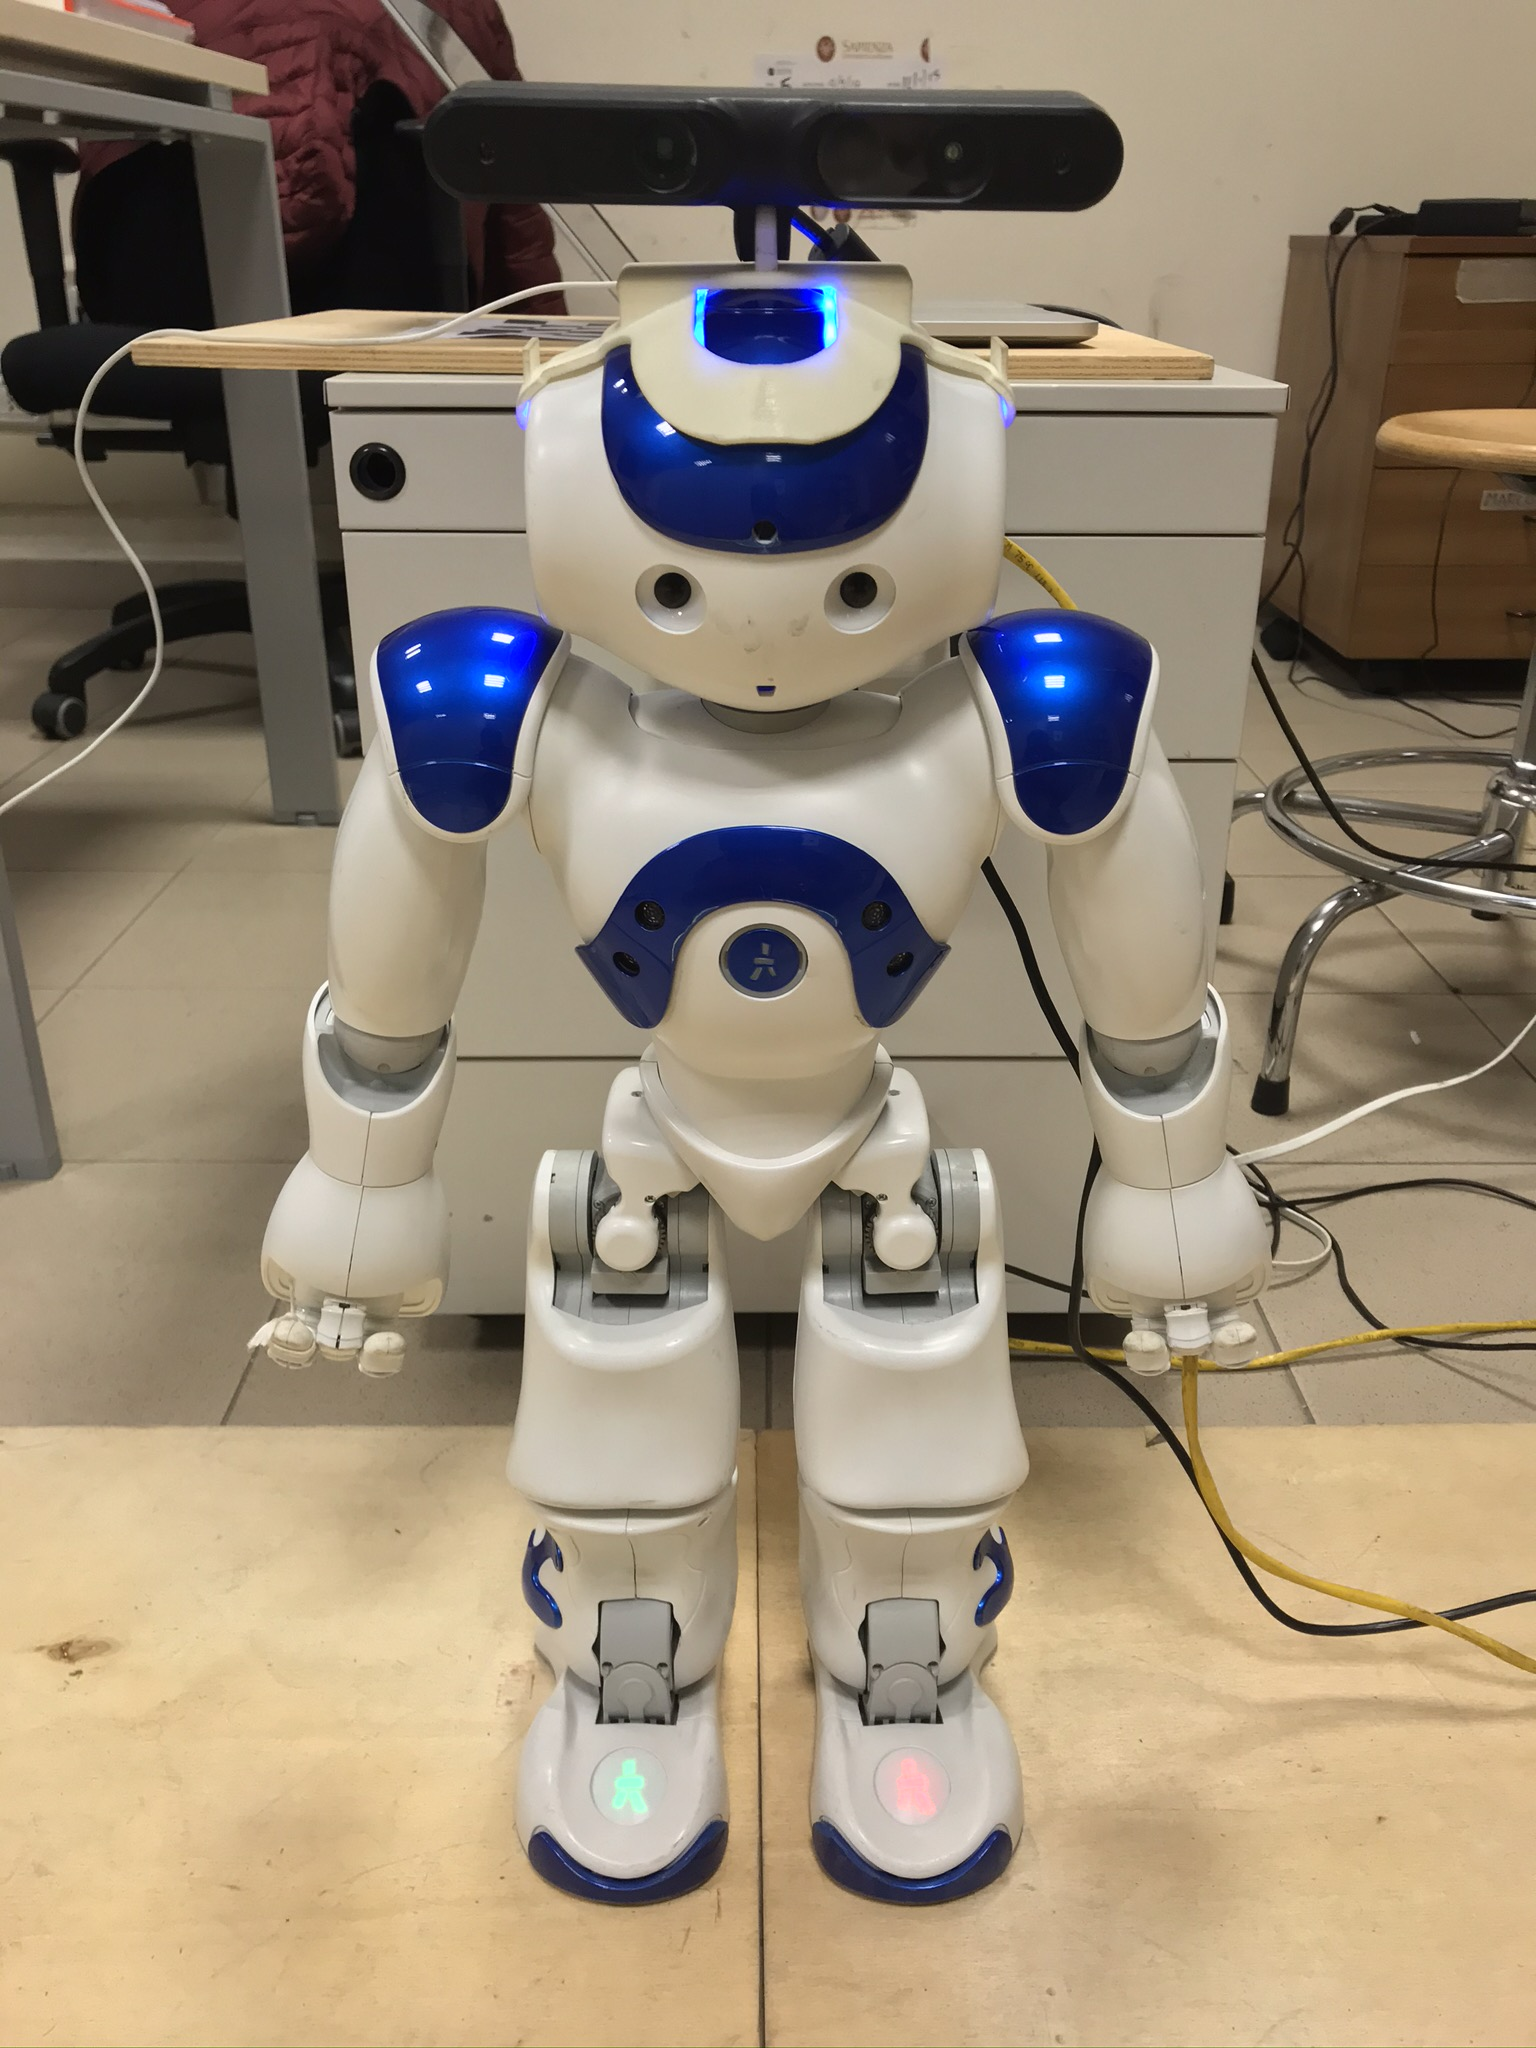
\includegraphics[width=\textwidth]{figures/NAO-with-xtion.JPEG}
        \caption{NAO with ASUS Xtion Pro placed on its head.}
    	\end{figure}		
	\end{columns}
\end{frame}

\begin{frame}{Stair Climbing in Unknown Environment}
	\begin{figure}
		\begin{subfigure}{0.40\textwidth}
			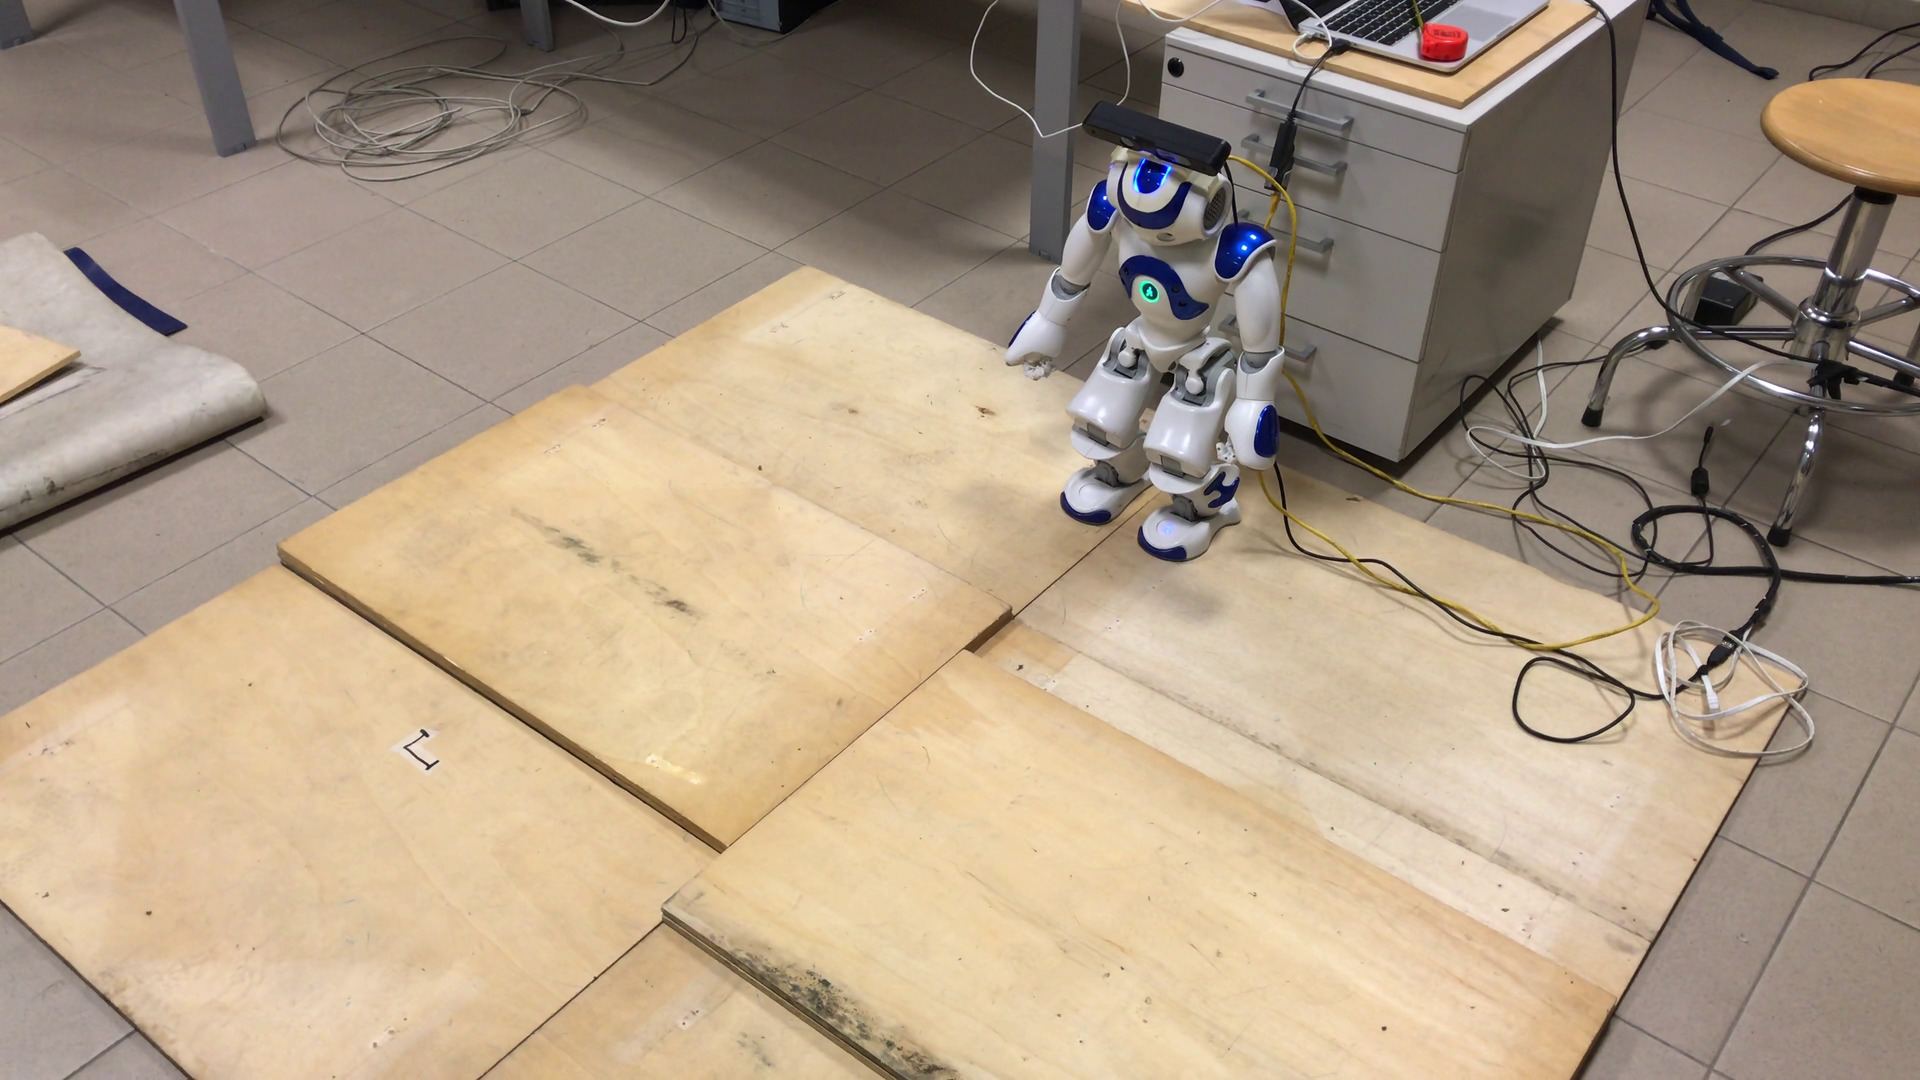
\includegraphics[width=\linewidth]
				{figures/experiments/unknown-env/video/01.jpeg}
			%\caption{Starting position}
		\end{subfigure}\hspace{0.05cm}%*{\fill}
		\begin{subfigure}{0.40\textwidth}
			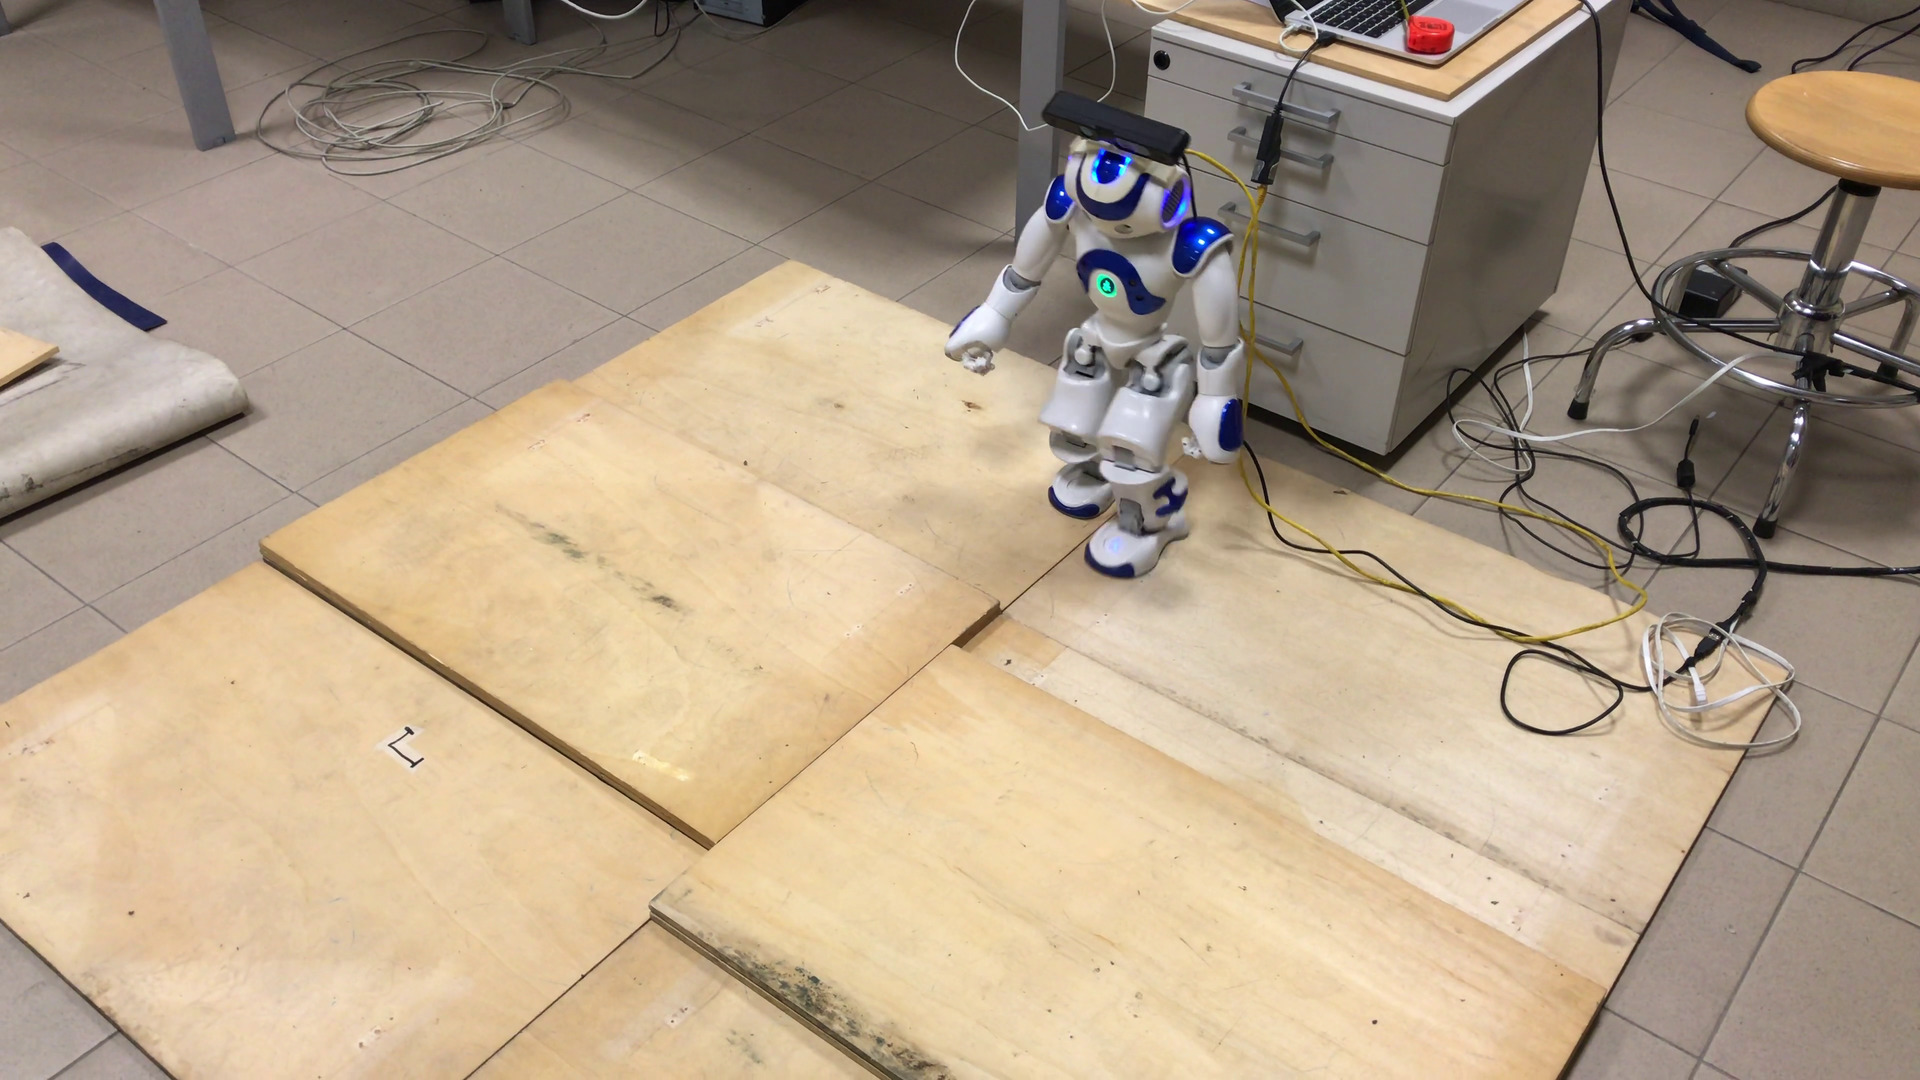
\includegraphics[width=\linewidth]
				{figures/experiments/unknown-env/video/02.jpeg}
			%\caption{First step}
		\end{subfigure}
		\begin{subfigure}{0.40\textwidth}
			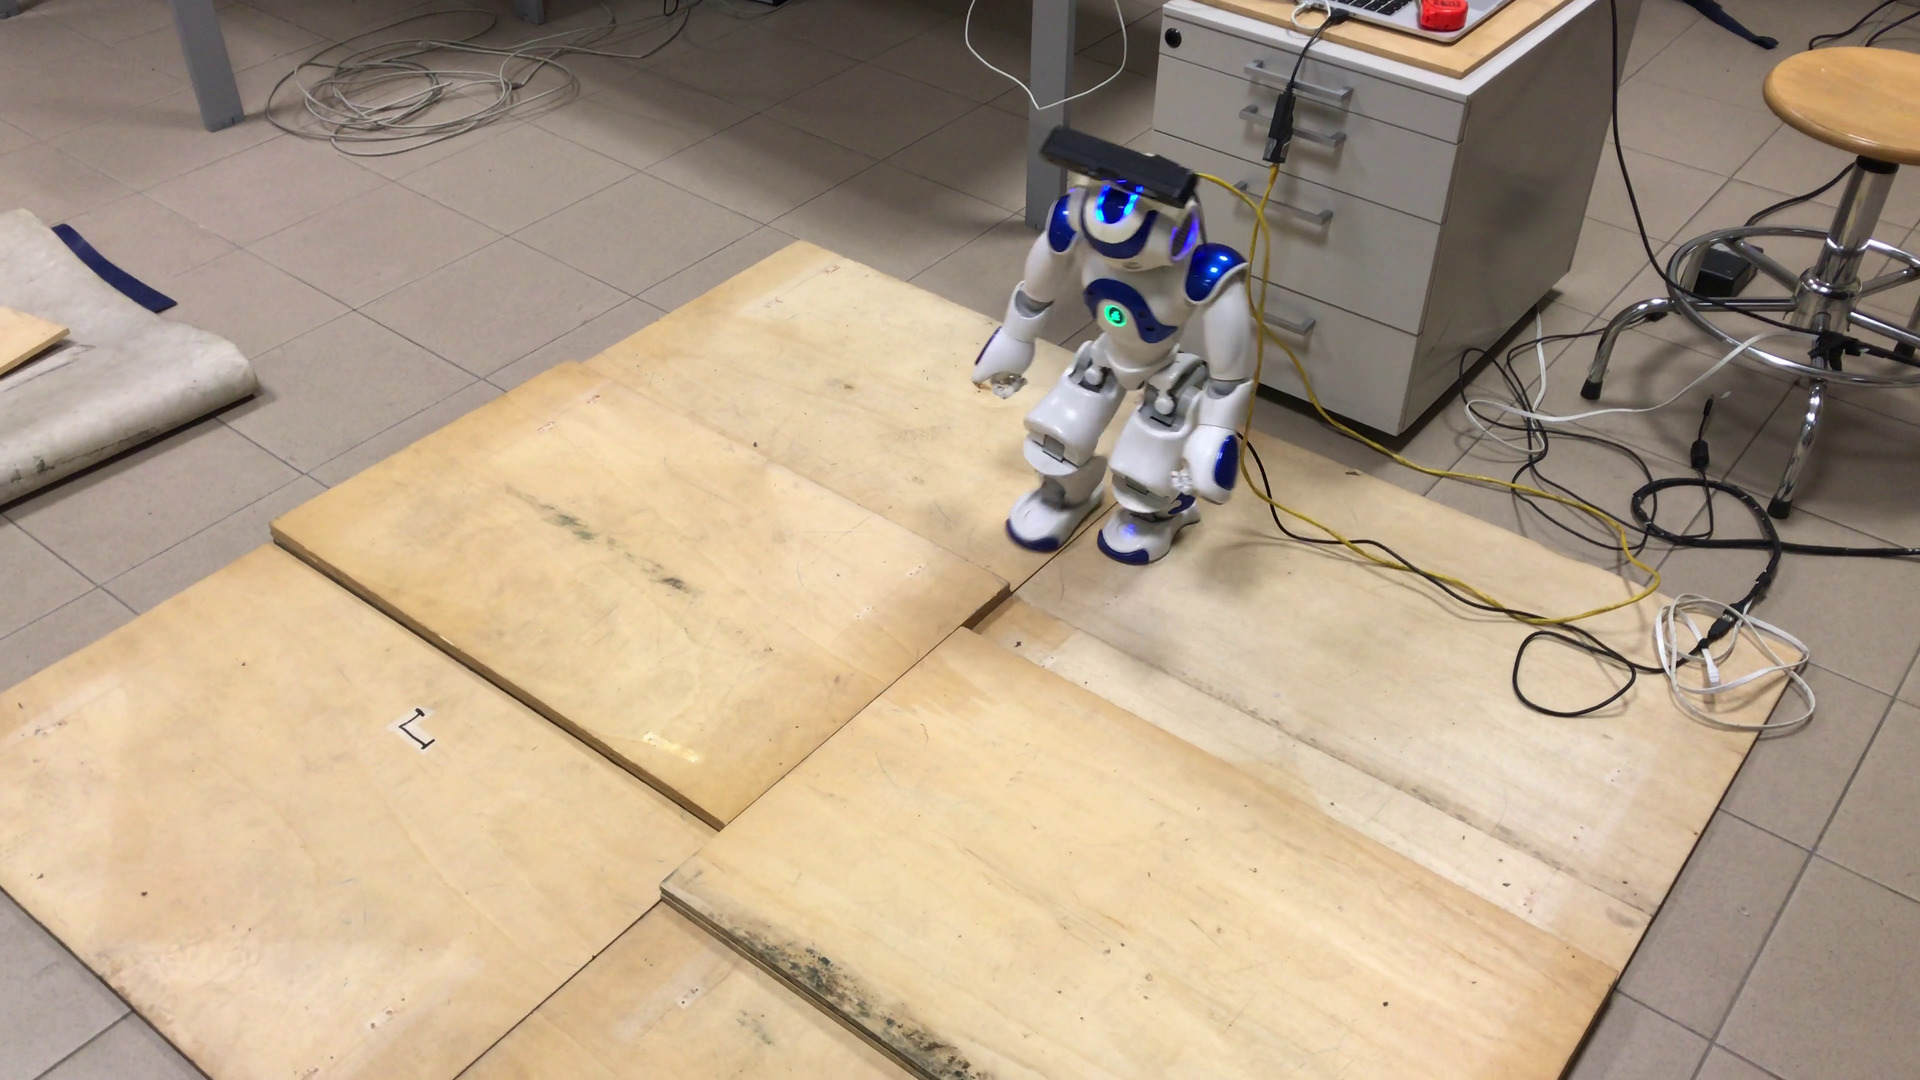
\includegraphics[width=\linewidth]
				{figures/experiments/unknown-env/video/03.jpeg}
			%\caption{Second step}
		\end{subfigure}\hspace{0.05cm}%*{\fill}
		\begin{subfigure}{0.40\textwidth}
			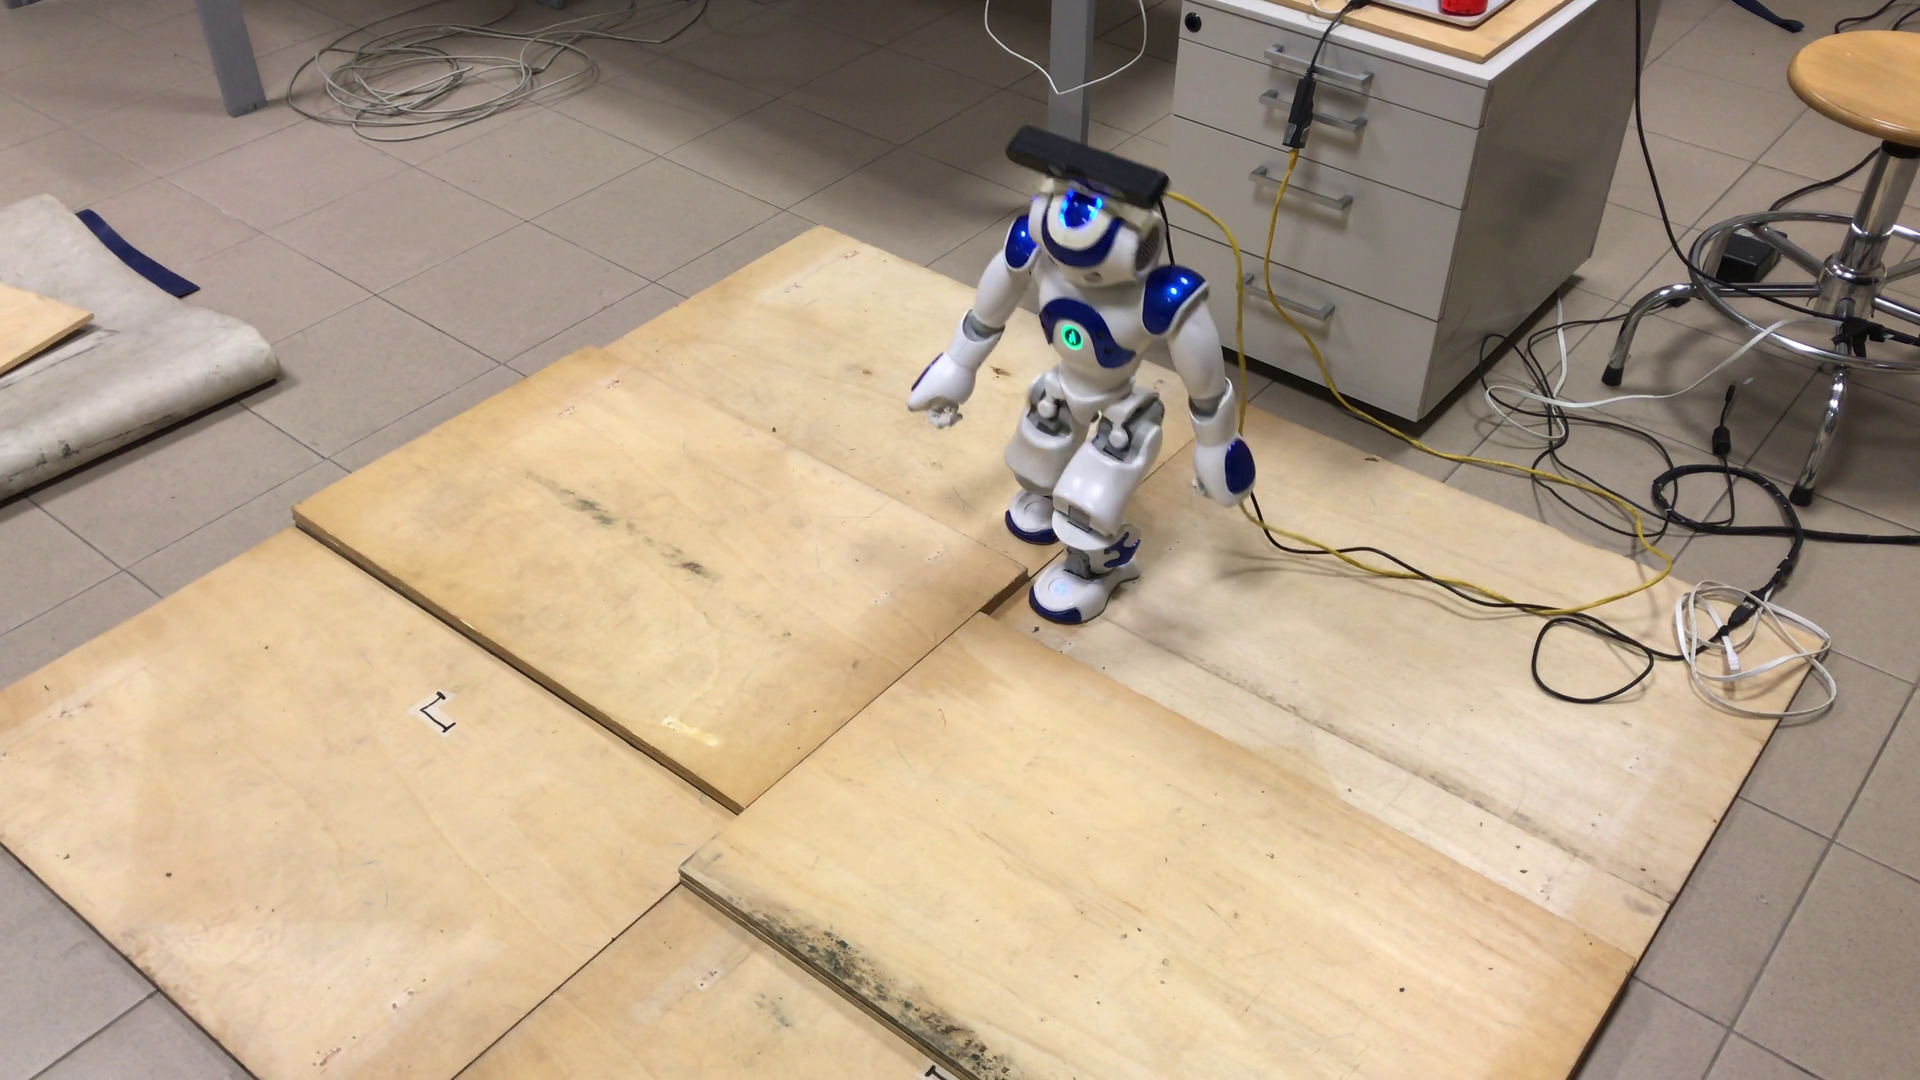
\includegraphics[width=\linewidth]
				{figures/experiments/unknown-env/video/04.jpeg}
			%\caption{Third step}
		\end{subfigure}
		\begin{subfigure}{0.40\textwidth}
			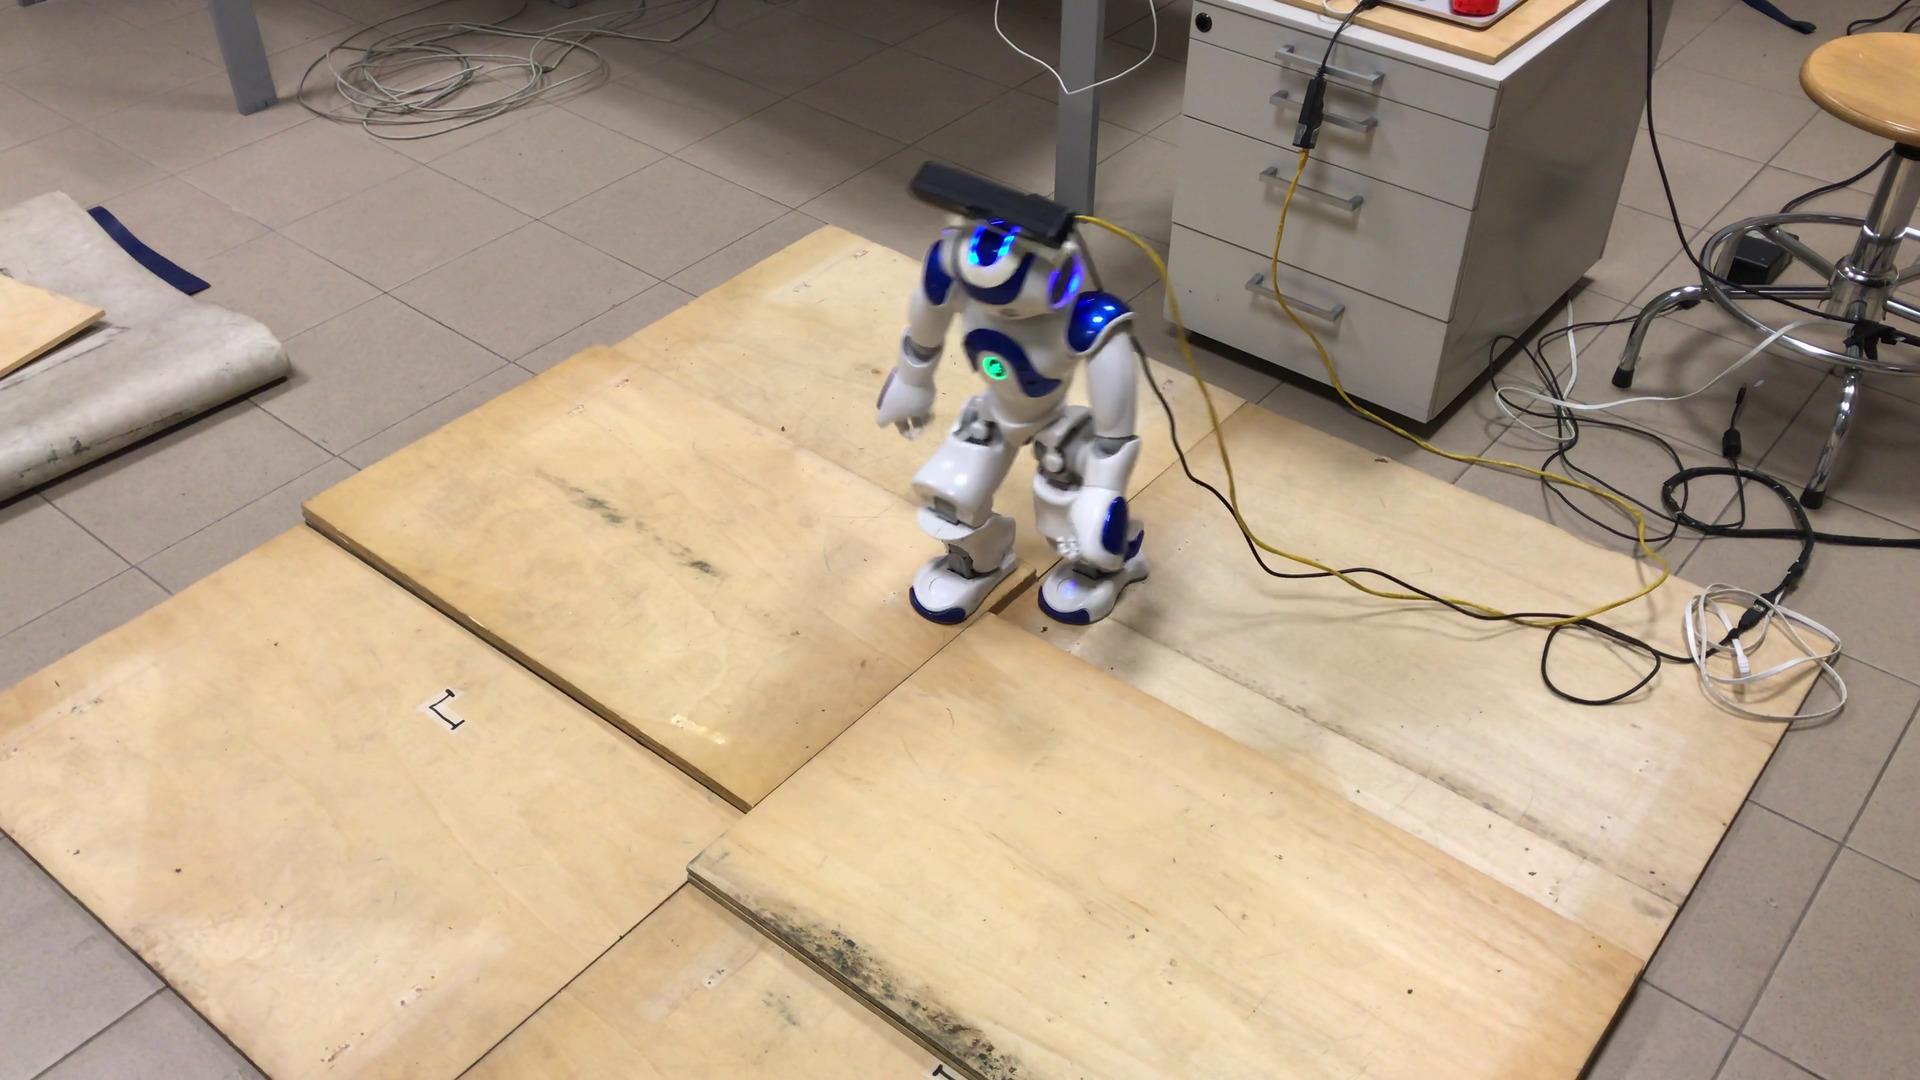
\includegraphics[width=\linewidth]
				{figures/experiments/unknown-env/video/05.jpeg}
			%\caption{Fourth step}
		\end{subfigure}\hspace{0.05cm}%*{\fill}
		\begin{subfigure}{0.40\textwidth}
			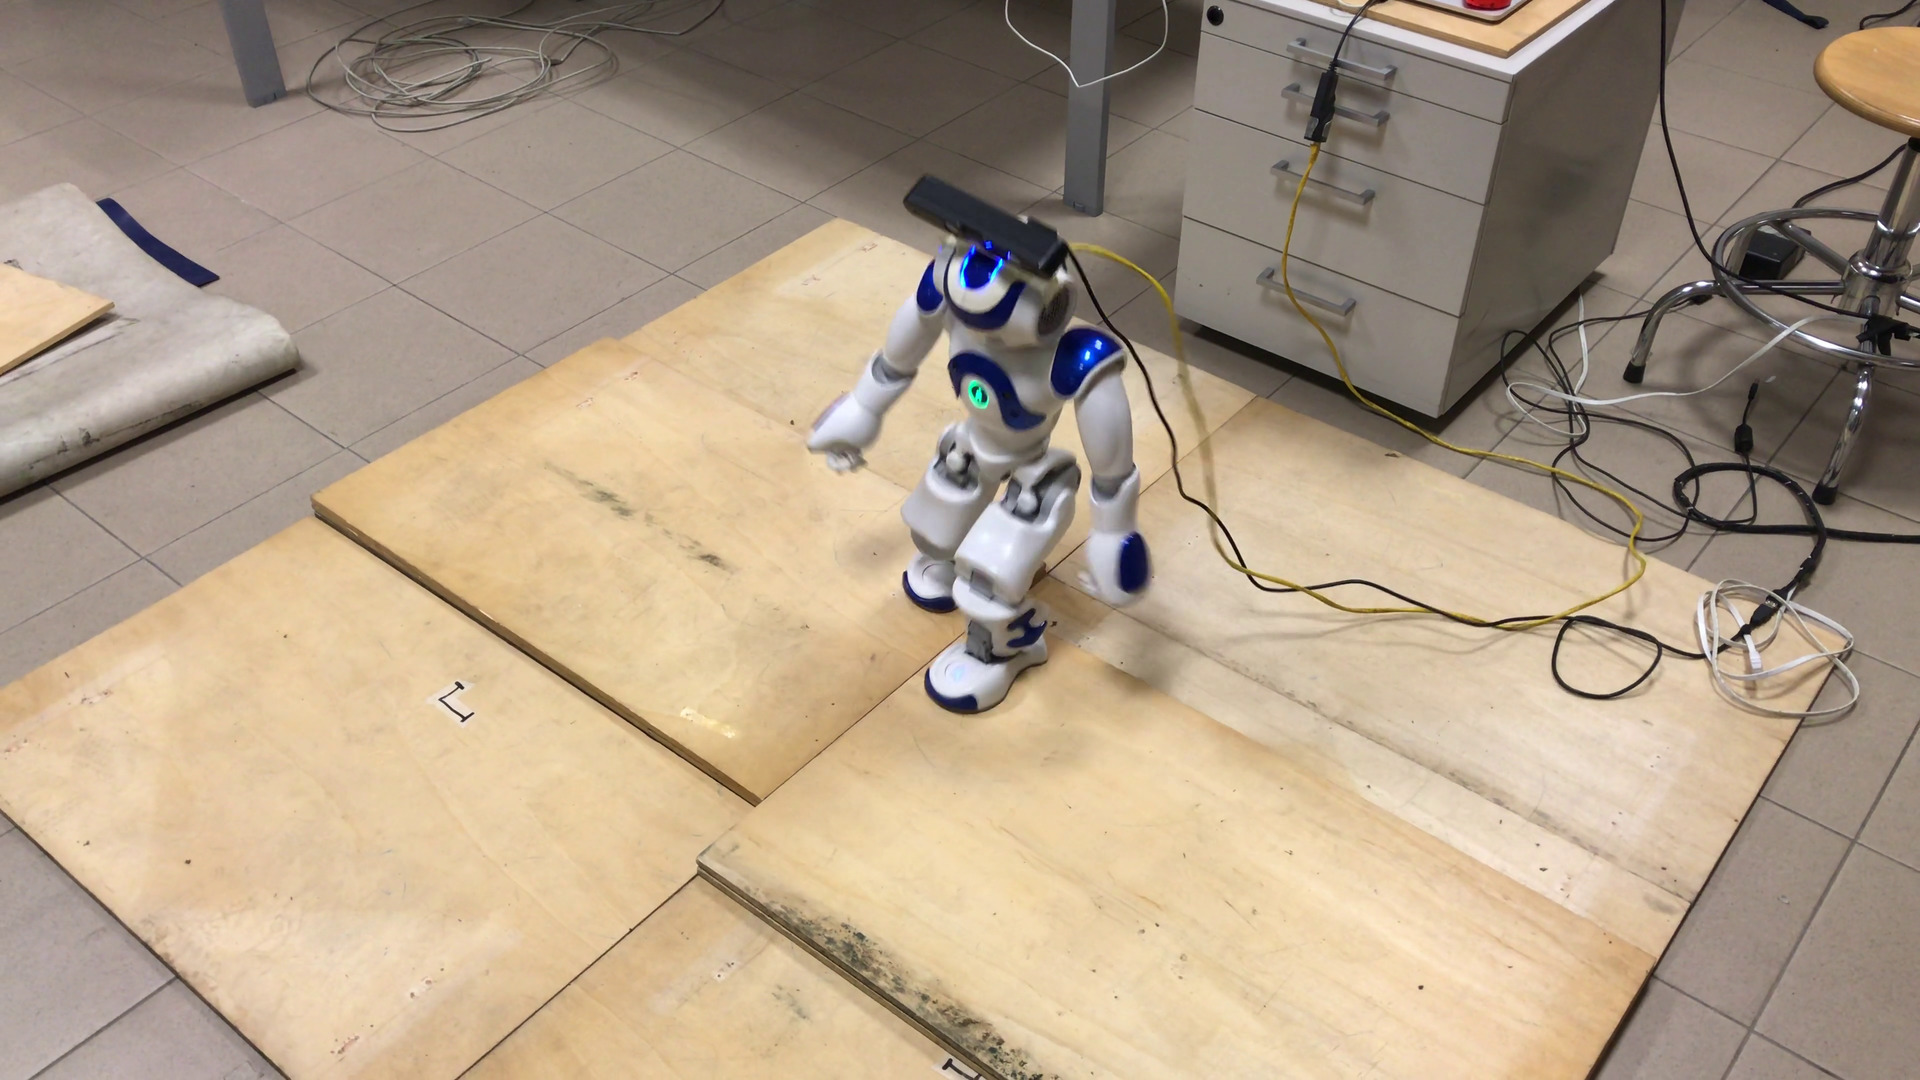
\includegraphics[width=\linewidth]
				{figures/experiments/unknown-env/video/06.jpeg}
			%\caption{Fifth step}
		\end{subfigure}
		\caption{NAO climbing the stairs in an unknown environment.}
	\end{figure}
\end{frame}

\begin{frame}{Stair Climbing in Unknown Environment: Footstep Plan}
	\begin{center}
    tree size: 454 -- solution size: 10 -- runtime: 331 ms
  \end{center}
	\begin{figure}
		\centering
		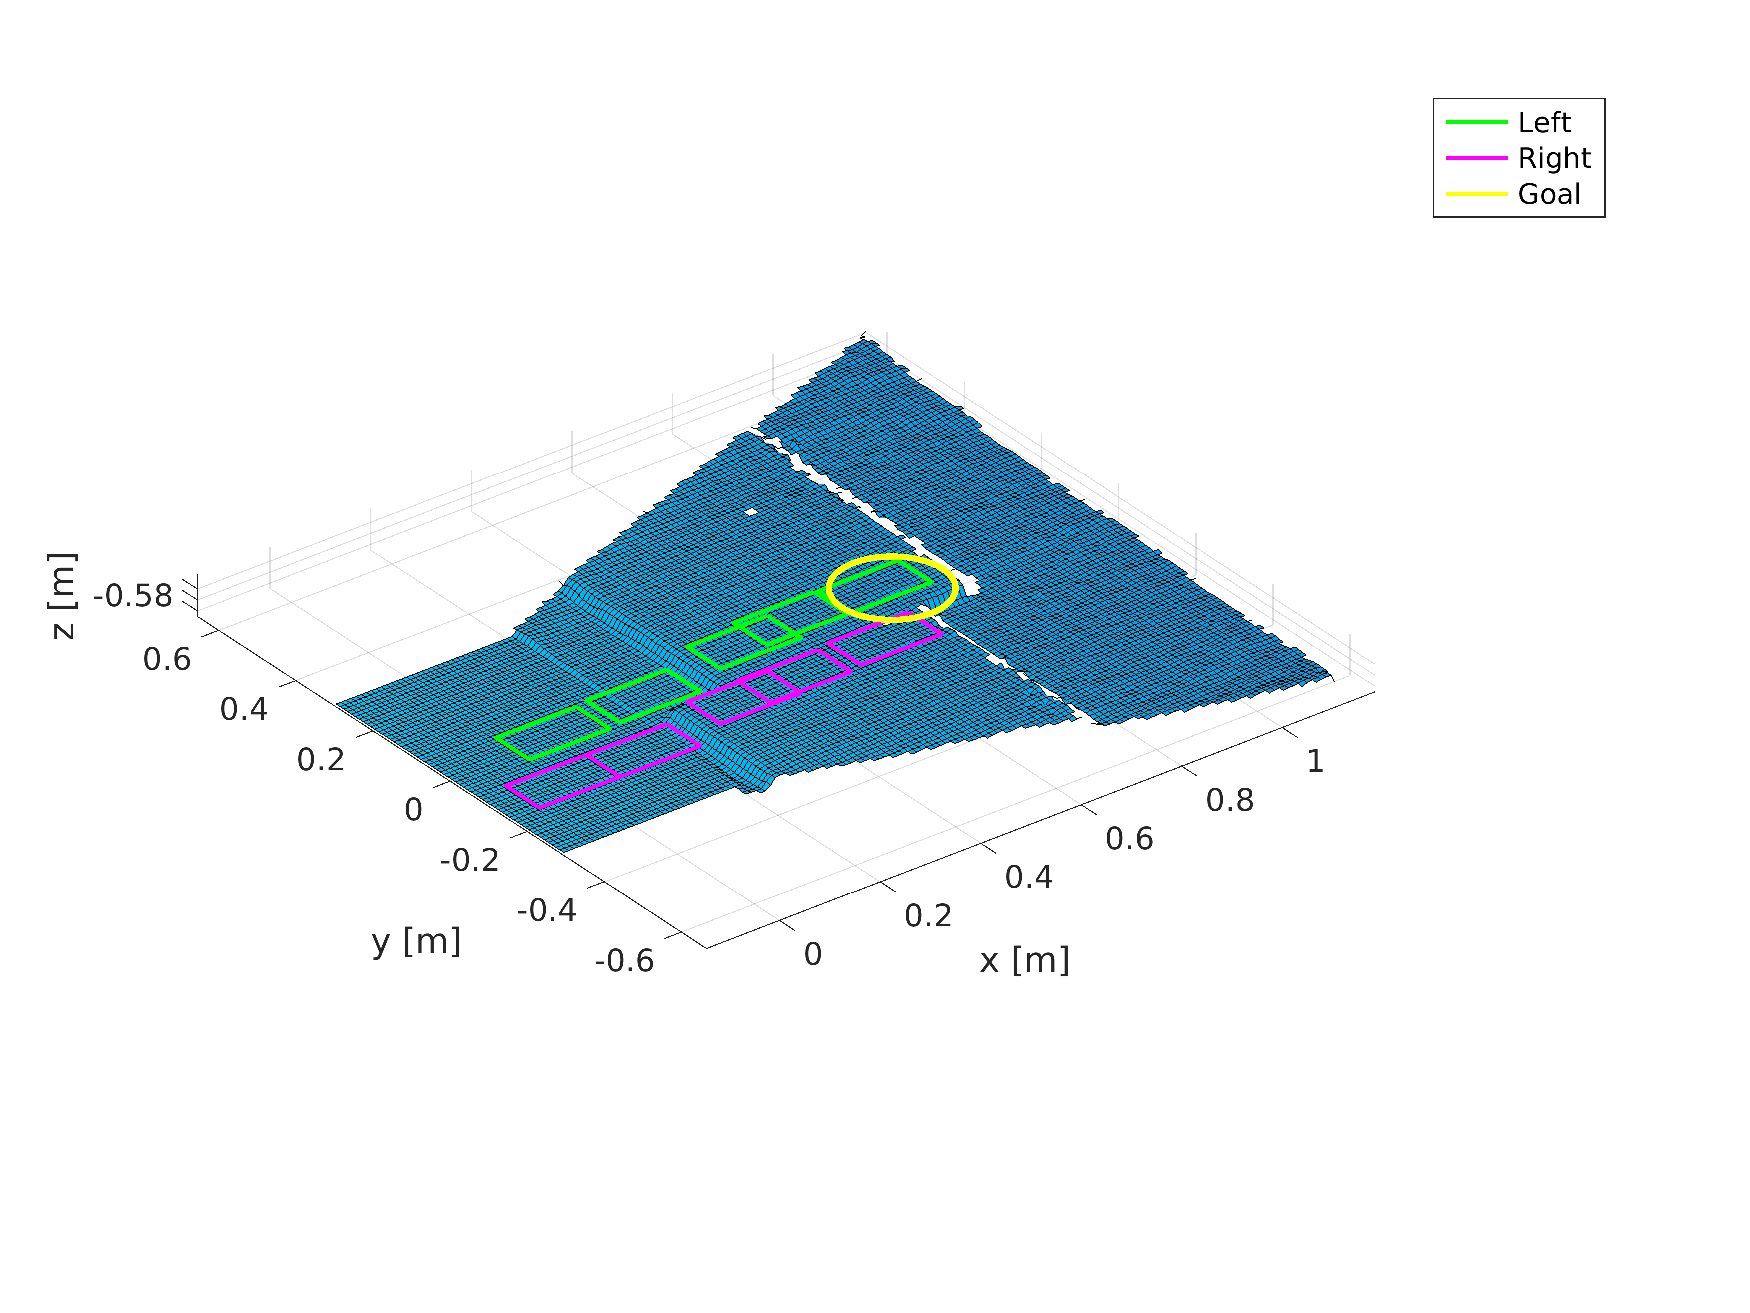
\includegraphics[width=0.8\textwidth]
				{figures/experiments/unknown-env/footstep-plan.pdf}
		\caption{Footstep plan generated for the scenario ``Stair Climbing in
				Unknown Environment''.}
	\end{figure}
\end{frame}

\begin{frame}[standout]
  Video
\end{frame}

\begin{frame}{Conclusion}
  Results. Future Works.
\end{frame}

\begin{frame}[standout]
    Q\&A
\end{frame}

\appendix

\begin{frame}{References}
  \bibliography{bibliography}
  \bibliographystyle{ieeetr}
\end{frame}

\end{document}

